\documentclass[11pt,a4paper]{article}
\usepackage[margin=22mm,headheight=15pt]{geometry}
\usepackage{graphicx,amsmath,amsfonts,booktabs,array,longtable,tabularx}
\usepackage{xcolor,fancyhdr,hyperref}
\definecolor{ink}{HTML}{20334B}
\definecolor{accent}{HTML}{245E91}
\hypersetup{colorlinks=true,linkcolor=accent,urlcolor=accent,pdftitle={Dimensionality reduction and autoencoders},pdfauthor={Group 32}}
\graphicspath{{figures/}}
\pagestyle{fancy}\fancyhf{}
\fancyhead[L]{\small CS601T: Deep Learning}
\fancyhead[R]{\small Assignment 4 / Group 32}
\fancyfoot[L]{\small MNIST digits 0, 3, 5, 6, 9}
\fancyfoot[R]{\thepage}
\setlength{\parindent}{0pt}\setlength{\parskip}{7pt}
\setlength{\emergencystretch}{2em}
\renewcommand{\arraystretch}{1.18}
\newcolumntype{Y}{>{\raggedright\arraybackslash}X}
\begin{document}

\hypersetup{pageanchor=false}

\begin{titlepage}\thispagestyle{empty}

{\color{accent}\large CS601T: Deep Learning}\par\vspace{24mm}

{\color{ink}\Huge\bfseries Dimensionality reduction\\and autoencoders}\par\vspace{8mm}

{\LARGE Programming Assignment 4}\par\vspace{4mm}

{\Large Group 32}\par\vspace{5mm}

{\large Autumn semester 2026}\par\vspace{10mm}

A complete six-task study using the supplied Group 32 MNIST subset. The report includes measured comparisons with an Assignment 3 reproduction trained on the same data splits.


\begingroup\small\setlength{\tabcolsep}{5pt}

\begin{tabularx}{\linewidth}{rY}

\toprule

\textbf{Task} & \textbf{Coverage} \\

\midrule

1 & PCA at 32, 64, 128, 256 dimensions; three FCNN architectures at every dimension \\

2 & Four shallow and four deep sigmoid autoencoders; final split reconstruction errors and examples \\

3 & Classification of all shallow autoencoder bottleneck representations \\

4 & Classification of all specified deep autoencoder bottleneck representations \\

5 & 20\% and 40\% masking denoising autoencoders; reconstruction and classification \\

6 & All encoder weight images for the selected shallow AE and both denoising AEs \\

\bottomrule\end{tabularx}\endgroup\par\medskip

All values are computed from saved results. No external digit images, pretrained models, or invented Assignment 3 measurements are used. The LaTeX source and local figures accompany this PDF.


\vfill\end{titlepage}\hypersetup{pageanchor=true}

\section{Dataset and experimental protocol}

\begingroup\small\setlength{\tabcolsep}{5pt}

\begin{tabularx}{\linewidth}{Yrrr}

\toprule

\textbf{Digit} & \textbf{Training} & \textbf{Validation} & \textbf{Test} \\

\midrule

0 & 2277 & 759 & 759 \\

3 & 2277 & 759 & 759 \\

5 & 2277 & 759 & 759 \\

6 & 2277 & 759 & 759 \\

9 & 2277 & 759 & 759 \\

Total & 11385 & 3795 & 3795 \\

\bottomrule\end{tabularx}\endgroup\par\medskip

Images are grayscale 28 $\times$ 28, flattened to 784 coordinates and divided by 255. Original train/validation/test splits are preserved. Internal class indices 0--4 map to digits 0, 3, 5, 6, and 9. Identical decoded pixel hashes overlap across splits in 0 cases.


\begingroup\small\setlength{\tabcolsep}{5pt}

\begin{tabularx}{\linewidth}{lY}

\toprule

\textbf{Setting} & \textbf{Assignment 4 value} \\

\midrule

Optimizer & Adam with learning rate 0.001 \\

Batch size & 256 \\

Epoch budget & Autoencoders at most 80; classifiers at most 40 \\

AE checkpoint / stopping & Minimum validation MSE; 12 stale epochs, after at least 20 epochs \\

FCNN checkpoint / stopping & Maximum validation accuracy; lower validation CE breaks ties; 8 stale epochs, after at least 12 epochs \\

FCNN features & Per-coordinate standardization fitted on the training representation only \\

FCNN architectures & 64; 128; 128 $\to$ 64 hidden neurons, ReLU, 5 output logits \\

Reproducibility & Base seed 32, deterministic CPU PyTorch, 4 threads \\

\bottomrule\end{tabularx}\endgroup\par\medskip

The same three FCNN architectures are considered in Tasks 1, 3, and 4. PCA, shallow, and deep classifiers use matching seeds for a given dimension and architecture. Digit labels enter classifier training only, not PCA fitting or the autoencoder loss.


\clearpage

\section{Model selection and Assignment 3 reference}

At each compressed dimension, validation accuracy selects an FCNN architecture and its saved checkpoint. Only that selected architecture is evaluated on the test set. The report then identifies the best observed test-ranked dimension as explicitly requested by the assignment. Such rankings are descriptive after dimension selection.


Assignment 3 is now reproduced from its supplied handout using three architectures with 3, 4, and 5 hidden layers and all seven prescribed optimizers. Every run uses the specified batch sizes, learning rate 0.001, identical initial weights within each architecture, and stopping criterion $|L_t-L_{t-1}|<10^{-4}$, without an epoch limit. The best converged architecture/optimizer is chosen by validation accuracy.


\begingroup\small\setlength{\tabcolsep}{5pt}

\begin{tabularx}{\linewidth}{lY}

\toprule

\textbf{Assignment 3 reference} & \textbf{Measured value} \\

\midrule

Architecture & 784 $\to$ 32 $\to$ 16 $\to$ 8 $\to$ 5 \\

Optimizer & NAG \\

Convergence epochs & 32 \\

Training accuracy & 99.99\% \\

Validation accuracy & 97.89\% \\

Test accuracy & 97.87\% \\

\bottomrule\end{tabularx}\endgroup\par\medskip

This is a newly measured reproduction, not a recovered historical submission. The earlier three-model raw-pixel reference did not meet Assignment 3's depth and optimizer requirements; it is no longer used as the Assignment 3 comparison. Assignment 3 and 4 share the same archive SHA-256 and exact split membership. Their architecture searches, optimizer schedules, and stopping rules differ as required by the respective handouts; the accuracy differences therefore compare these studies rather than isolate compression alone.


\clearpage

\section{Task 1: PCA and classification}

PCA is fitted by exact eigendecomposition of the training sample covariance. The training mean centers every split; validation and test images do not fit the directions or mean.


\[\mu=\frac{1}{N_{\rm tr}}\sum_i x_i,\quad C=\frac{(X_{\rm tr}-\mu)^T(X_{\rm tr}-\mu)}{N_{\rm tr}-1},\quad Z_s=(X_s-\mu)V_d.\]

\begingroup\small\setlength{\tabcolsep}{5pt}

\begin{tabularx}{\linewidth}{rYYYlr}

\toprule

\textbf{Dim.} & \textbf{Val: 64} & \textbf{Val: 128} & \textbf{Val: 128--64} & \textbf{Selected} & \textbf{Test} \\

\midrule

32 & 97.81\% & 98.31\% & 98.16\% & 128 & 97.81\% \\

64 & 97.94\% & 98.21\% & 97.71\% & 128 & 98.18\% \\

128 & 97.50\% & 97.71\% & 97.55\% & 128 & 97.58\% \\

256 & 96.76\% & 97.02\% & 96.39\% & 128 & 97.10\% \\

\bottomrule\end{tabularx}\endgroup\par\medskip

\begingroup\small\setlength{\tabcolsep}{5pt}

\begin{tabularx}{\linewidth}{Yr}

\toprule

\textbf{Dimension} & \textbf{Training variance retained} \\

\midrule

32 & 76.11\% \\

64 & 87.00\% \\

128 & 93.88\% \\

256 & 98.01\% \\

\bottomrule\end{tabularx}\endgroup\par\medskip

Larger dimensions retain more training variance, but variance preservation is not the same objective as discrimination. In particular, the FCNN's training-fitted coordinate scaling gives each retained component unit training variance.


The highest observed test result is \textbf{98.18\%} at \textbf{64 dimensions}, with FCNN hidden layers 128. It differs from the Assignment 3 reference by +0.32 percentage points.


\clearpage

\section{Task 1: test confusion matrices}

\begin{center}

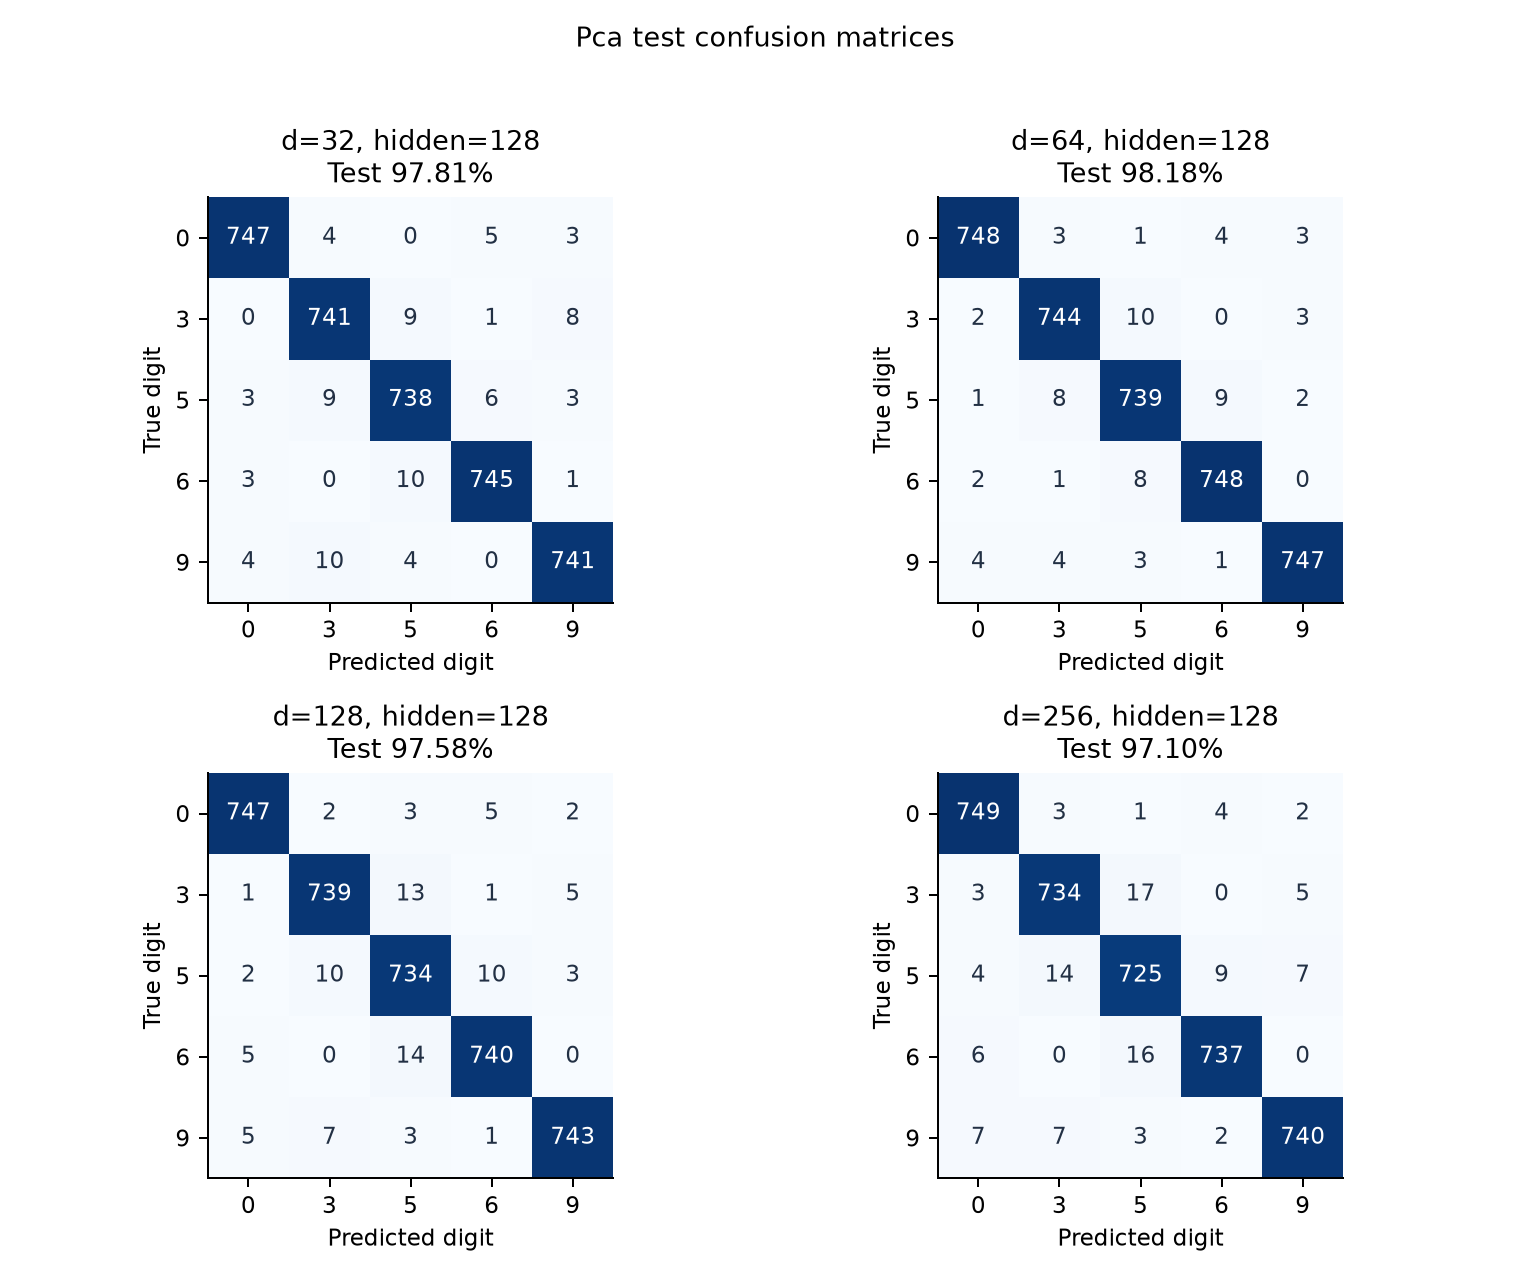
\includegraphics[width=\linewidth,height=0.73\textheight,keepaspectratio]{confusion_pca.png}

\end{center}

{\small Rows are true digits; columns are predicted digits. Each row contains 759 test images. One matrix is provided for the validation-selected FCNN at each dimension.}\par

At the test-ranked best dimension, the largest directional confusion is digit 3 predicted as 5 (10 images).


\clearpage

\section{Task 2: image reconstruction}

For each bottleneck width $d\in\{32,64,128,256\}$, the shallow autoencoder is $784\to d\to784$, and the deep autoencoder is $784\to400\to d\to400\to784$. Logistic sigmoid is used in every hidden layer and the reconstruction output. Adam minimizes pixelwise MSE.


\[\mathrm{MSE}_s=\frac{1}{N_s\,784}\sum_{i=1}^{N_s}\sum_{j=1}^{784}\bigl(\hat{x}_{ij}-x_{ij}\bigr)^2.\]

The validation-selected checkpoint is restored before computing the complete split averages. To express error as average squared Euclidean error per image, multiply the listed MSE by 784.


\begingroup\small\setlength{\tabcolsep}{5pt}

\begin{tabularx}{\linewidth}{Yrrrr}

\toprule

\textbf{Autoencoder} & \textbf{Epoch} & \textbf{Train MSE} & \textbf{Val MSE} & \textbf{Test MSE} \\

\midrule

shallow\_32 & 80 & 0.032662 & 0.033074 & 0.033134 \\

shallow\_64 & 80 & 0.017536 & 0.018082 & 0.018146 \\

shallow\_128 & 80 & 0.006686 & 0.007328 & 0.007351 \\

shallow\_256 & 80 & 0.002846 & 0.003380 & 0.003395 \\

deep\_32 & 80 & 0.013783 & 0.014634 & 0.014712 \\

deep\_64 & 80 & 0.011083 & 0.012002 & 0.012069 \\

deep\_128 & 80 & 0.009426 & 0.010395 & 0.010428 \\

deep\_256 & 80 & 0.008086 & 0.009112 & 0.009136 \\

\bottomrule\end{tabularx}\endgroup\par\medskip

The lowest test reconstruction MSE is 0.003395 for shallow\_256. Reconstruction and classification optimize different objectives; a low pixel loss need not imply the highest digit accuracy.


\clearpage

\section{Task 2: train reconstruction examples}

\begin{center}

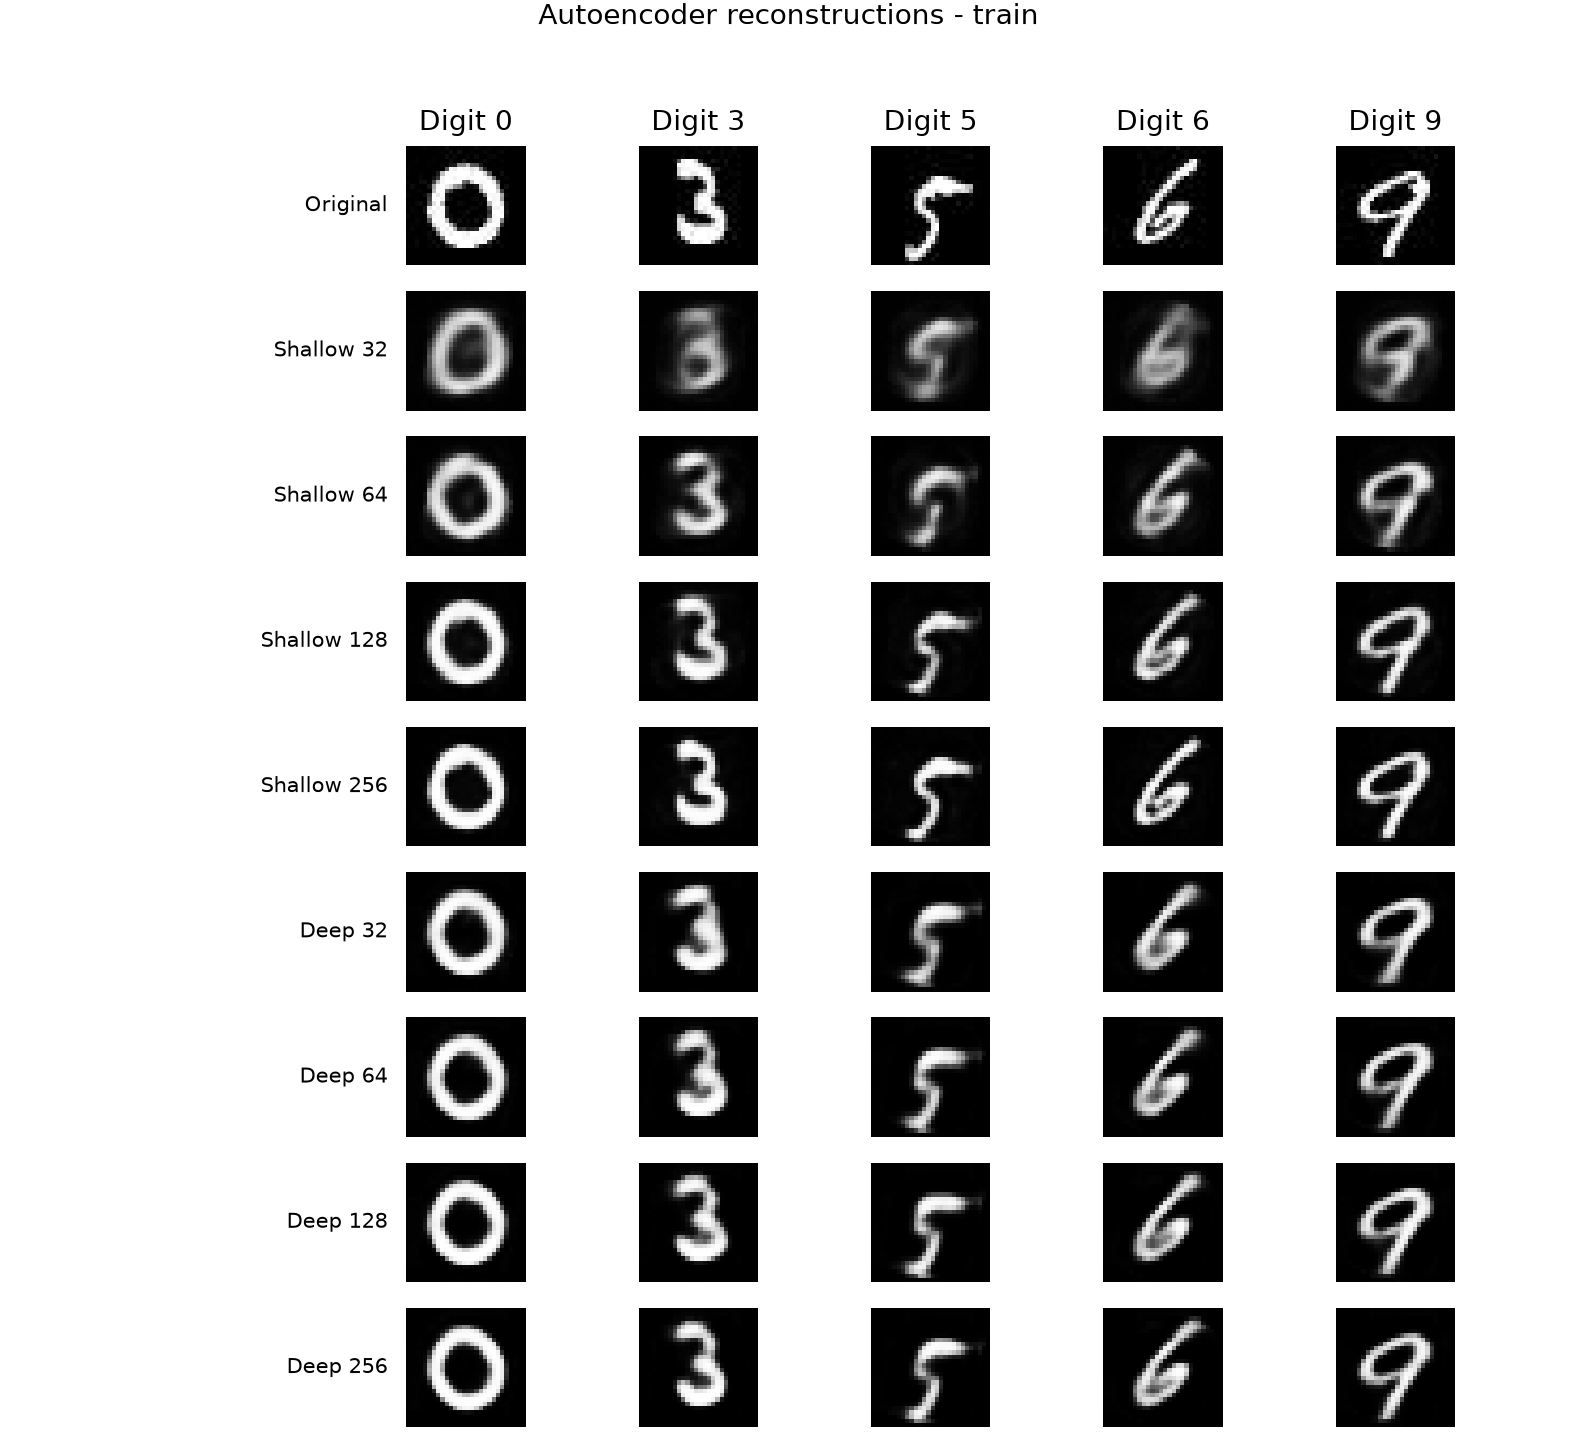
\includegraphics[width=\linewidth,height=0.80\textheight,keepaspectratio]{reconstructions_train.png}

\end{center}

{\small One deterministic image per class from this split is used for every architecture. The first row is original; the remaining eight rows show shallow and deep reconstructions. The same images are reused in Task 5.}\par

\clearpage

\section{Task 2: val reconstruction examples}

\begin{center}

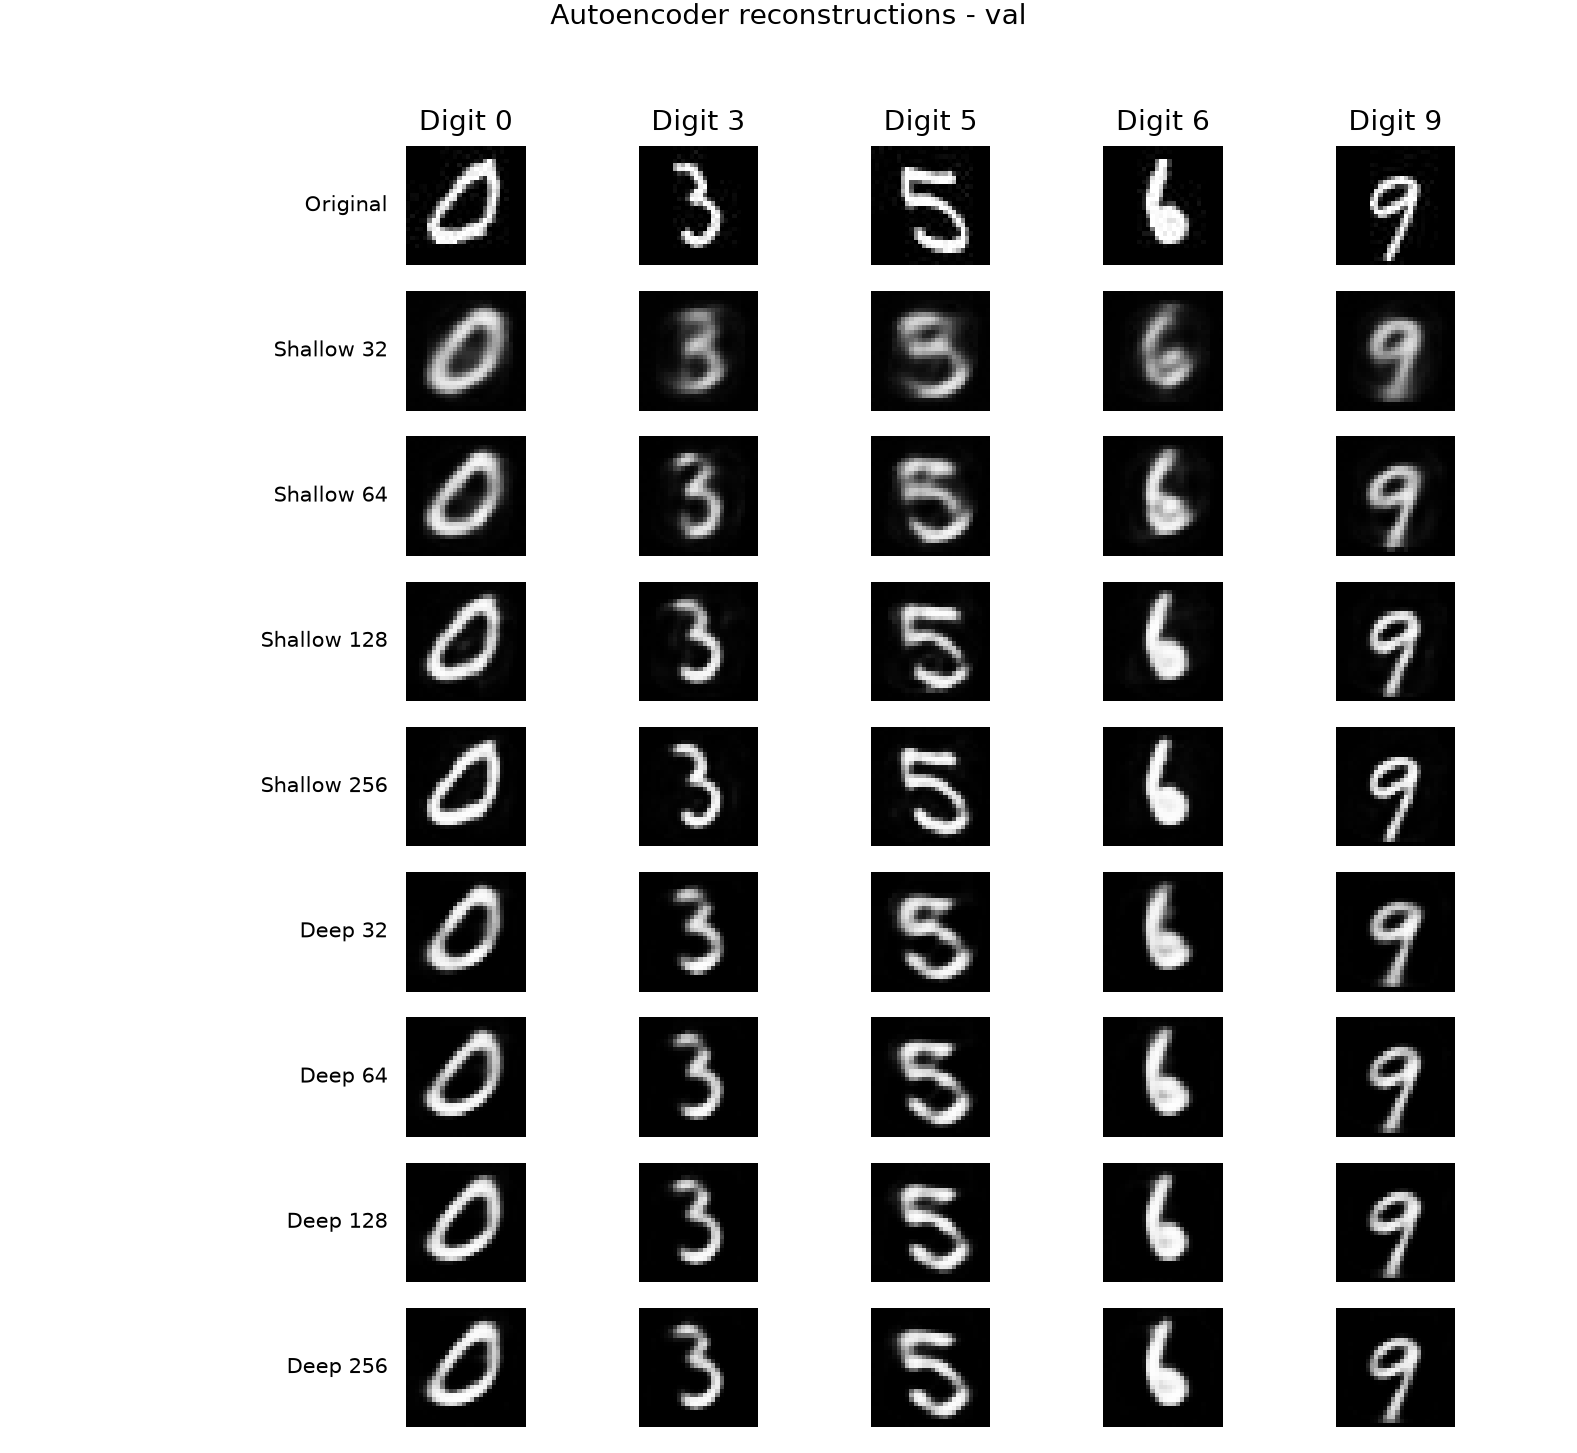
\includegraphics[width=\linewidth,height=0.80\textheight,keepaspectratio]{reconstructions_val.png}

\end{center}

{\small One deterministic image per class from this split is used for every architecture. The first row is original; the remaining eight rows show shallow and deep reconstructions. The same images are reused in Task 5.}\par

\clearpage

\section{Task 2: test reconstruction examples}

\begin{center}

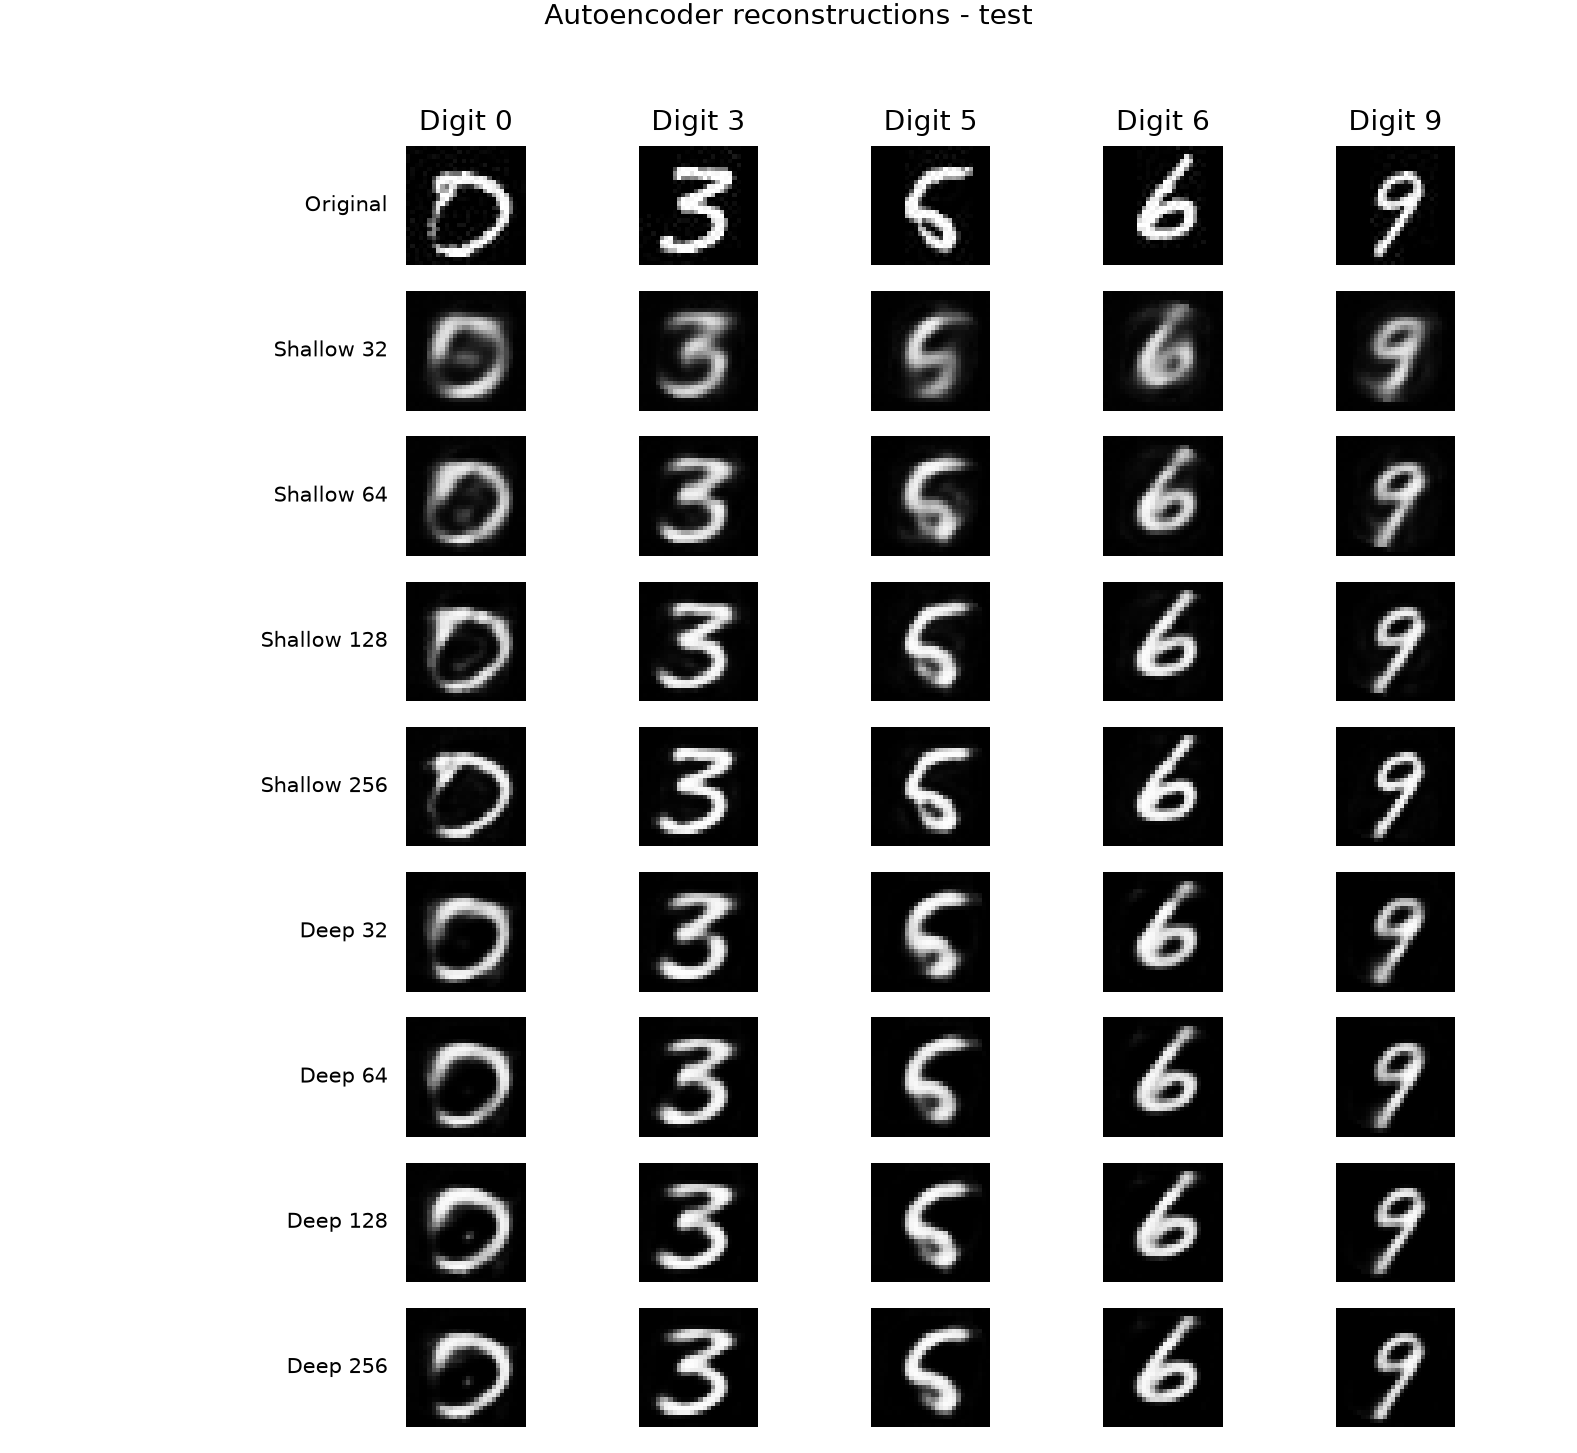
\includegraphics[width=\linewidth,height=0.80\textheight,keepaspectratio]{reconstructions_test.png}

\end{center}

{\small One deterministic image per class from this split is used for every architecture. The first row is original; the remaining eight rows show shallow and deep reconstructions. The same images are reused in Task 5.}\par

\clearpage

\section{Task 3: shallow autoencoder representations}

The trained encoder is frozen. Training, validation, and test images are passed through it, and the sigmoid bottleneck output is saved as the compressed representation. Training-fitted standardization precedes the separate supervised FCNN; the saved latent codes themselves are unstandardized.


\begingroup\small\setlength{\tabcolsep}{5pt}

\begin{tabularx}{\linewidth}{rYYYlr}

\toprule

\textbf{Dim.} & \textbf{Val: 64} & \textbf{Val: 128} & \textbf{Val: 128--64} & \textbf{Selected} & \textbf{Test} \\

\midrule

32 & 94.91\% & 95.42\% & 95.44\% & 128 $\to$ 64 & 95.60\% \\

64 & 96.68\% & 97.31\% & 97.52\% & 128 $\to$ 64 & 97.34\% \\

128 & 97.89\% & 98.08\% & 97.94\% & 128 & 97.81\% \\

256 & 97.81\% & 98.10\% & 98.21\% & 128 $\to$ 64 & 98.05\% \\

\bottomrule\end{tabularx}\endgroup\par\medskip

The highest observed test result is \textbf{98.05\%} at \textbf{256 dimensions}, with FCNN hidden layers 128 $\to$ 64. It differs from the Assignment 3 reference by +0.18 percentage points.


The difference from the best PCA test accuracy is -0.13 percentage points.


\clearpage

\section{Task 3: test confusion matrices}

\begin{center}

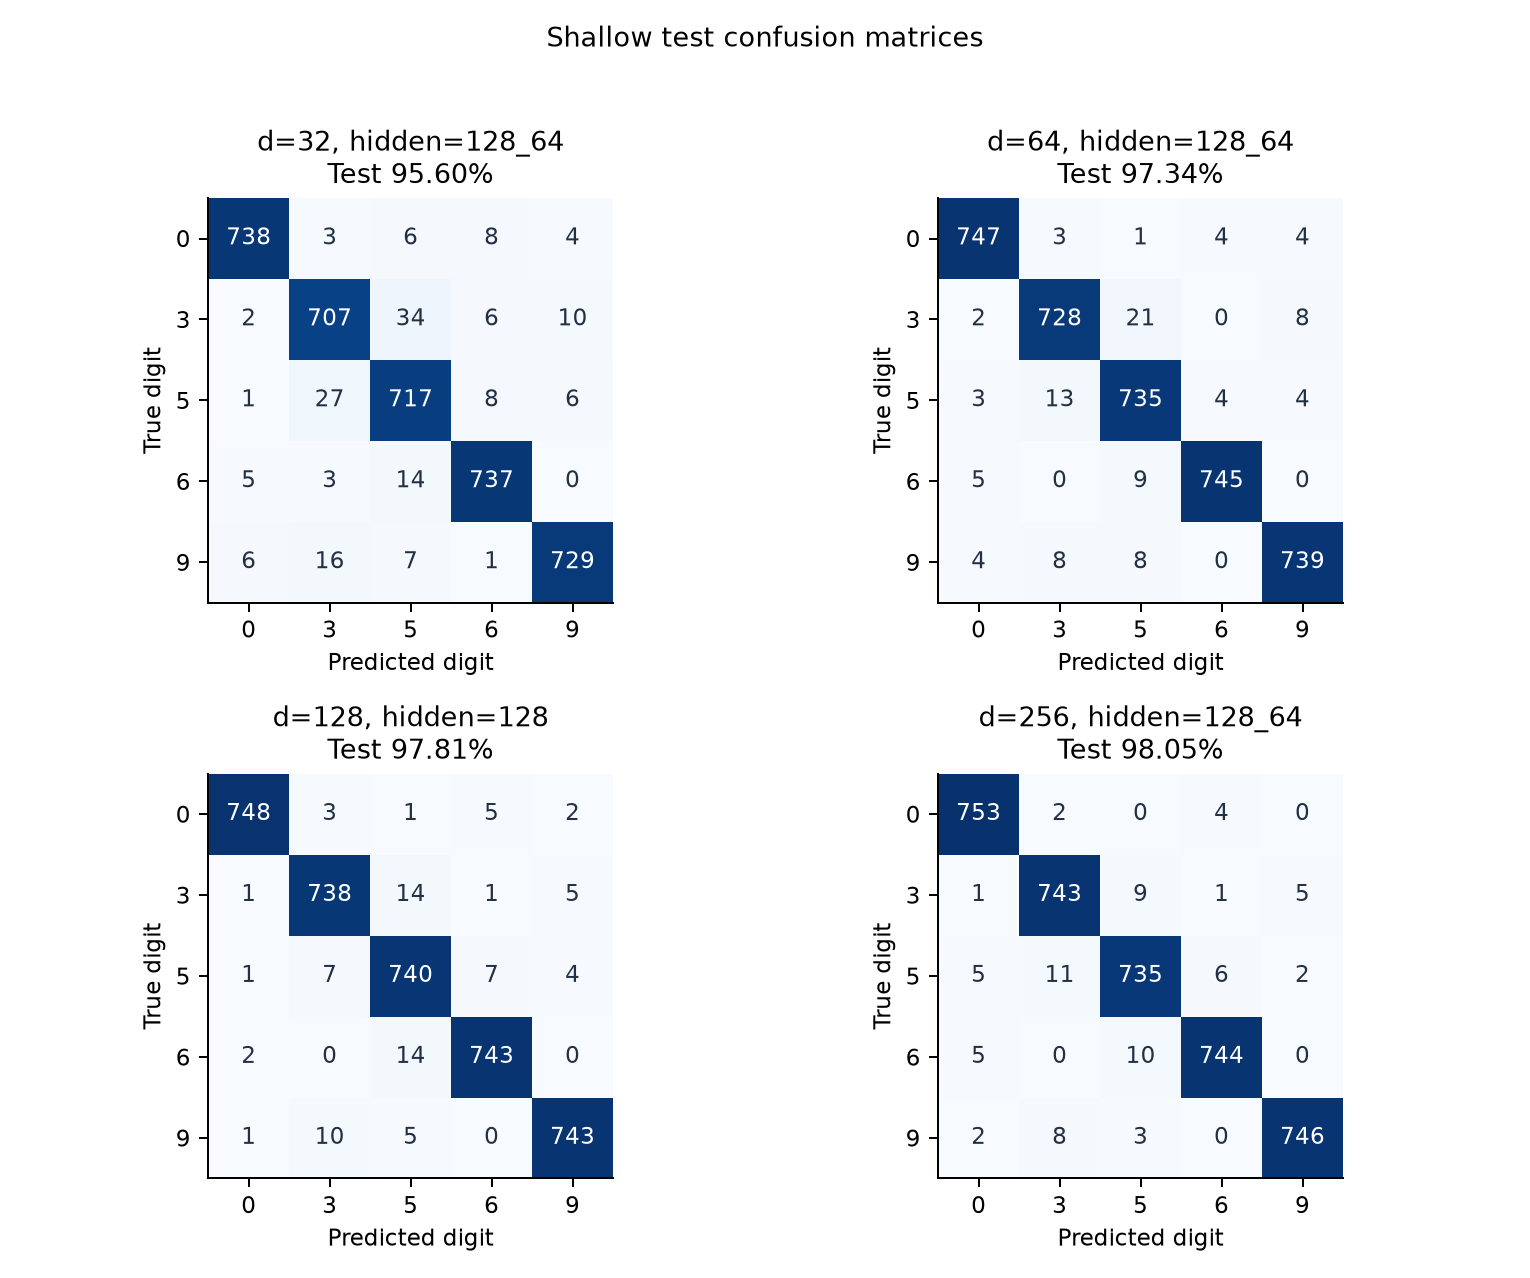
\includegraphics[width=\linewidth,height=0.73\textheight,keepaspectratio]{confusion_shallow.png}

\end{center}

{\small Rows are true digits; columns are predicted digits. Each row contains 759 test images. One matrix is provided for the validation-selected FCNN at each dimension.}\par

At the test-ranked best dimension, the largest directional confusion is digit 5 predicted as 3 (11 images).


\clearpage

\section{Task 4: deep autoencoder representations}

The trained encoder is frozen. Training, validation, and test images are passed through it, and the sigmoid bottleneck output is saved as the compressed representation. Training-fitted standardization precedes the separate supervised FCNN; the saved latent codes themselves are unstandardized.


\begingroup\small\setlength{\tabcolsep}{5pt}

\begin{tabularx}{\linewidth}{rYYYlr}

\toprule

\textbf{Dim.} & \textbf{Val: 64} & \textbf{Val: 128} & \textbf{Val: 128--64} & \textbf{Selected} & \textbf{Test} \\

\midrule

32 & 97.39\% & 97.76\% & 97.84\% & 128 $\to$ 64 & 97.58\% \\

64 & 98.00\% & 97.97\% & 98.23\% & 128 $\to$ 64 & 98.13\% \\

128 & 98.29\% & 98.47\% & 98.42\% & 128 & 98.16\% \\

256 & 98.23\% & 98.63\% & 98.52\% & 128 & 98.18\% \\

\bottomrule\end{tabularx}\endgroup\par\medskip

The highest observed test result is \textbf{98.18\%} at \textbf{256 dimensions}, with FCNN hidden layers 128. It differs from the Assignment 3 reference by +0.32 percentage points.


The difference from the best PCA test accuracy is +0.00 percentage points.


The difference from the best shallow AE classification test accuracy is +0.13 percentage points.


\clearpage

\section{Task 4: test confusion matrices}

\begin{center}

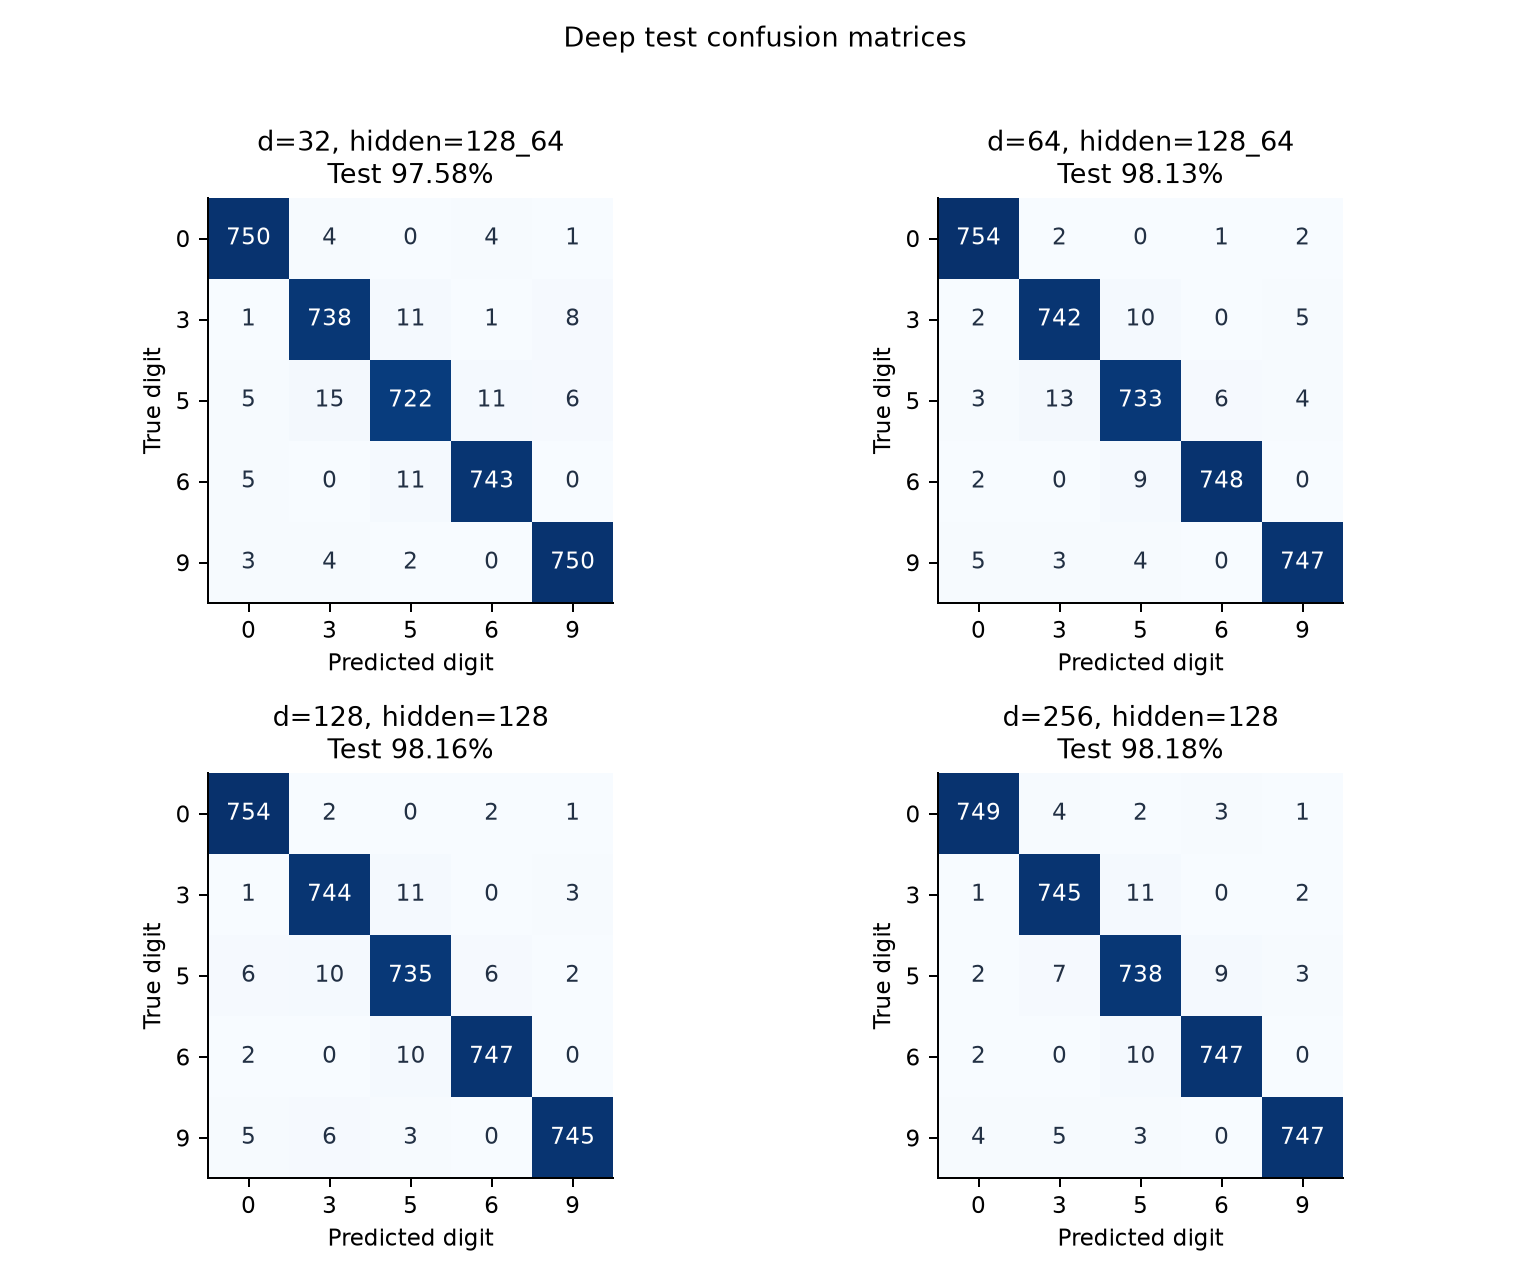
\includegraphics[width=\linewidth,height=0.73\textheight,keepaspectratio]{confusion_deep.png}

\end{center}

{\small Rows are true digits; columns are predicted digits. Each row contains 759 test images. One matrix is provided for the validation-selected FCNN at each dimension.}\par

At the test-ranked best dimension, the largest directional confusion is digit 3 predicted as 5 (11 images).


\clearpage

\section{Task 5: denoising autoencoders}

The brief requires selecting the bottleneck using Task 3's best test accuracy. This selects $d=256$. Both denoising autoencoders use $784\to256\to784$, sigmoid activations, and Adam. Their FCNN uses the same best Task 3 hidden architecture at that dimension: 128 $\to$ 64.


Noise is independent Bernoulli pixel masking. A selected pixel is set to zero with probability 0.20 or 0.40; the clean image is the target. Training samples fresh masks in every batch. Fixed independently seeded masks are used for post-training split errors and example images. Percentages denote expected masking rates.


\[\tilde{x}=m\odot x,\qquad m_j\sim\operatorname{Bernoulli}(1-p),\qquad \min_\theta\;\mathbb{E}_{x,m}\lVert f_\theta(\tilde{x})-x\rVert_2^2.\]

\begingroup\small\setlength{\tabcolsep}{5pt}

\begin{tabularx}{\linewidth}{Yrrrr}

\toprule

\textbf{Masking} & \textbf{Epoch} & \textbf{Train MSE} & \textbf{Val MSE} & \textbf{Test MSE} \\

\midrule

20\% & 80 & 0.007776 & 0.008404 & 0.008378 \\

40\% & 80 & 0.011865 & 0.012494 & 0.012545 \\

\bottomrule\end{tabularx}\endgroup\par\medskip

These errors reconstruct clean targets from the fixed corrupted inputs. For clean inputs, validation/test MSE are 20\%: 0.007596 / 0.007598; 40\%: 0.015163 / 0.015130.


\begingroup\small\setlength{\tabcolsep}{5pt}

\begin{tabularx}{\linewidth}{lYrrrr}

\toprule

\textbf{Masking} & \textbf{FCNN} & \textbf{Clean val.} & \textbf{Clean test} & \textbf{Noisy val.} & \textbf{Noisy test} \\

\midrule

20\% & 128 $\to$ 64 & 98.10\% & 97.71\% & 97.47\% & 97.31\% \\

40\% & 128 $\to$ 64 & 98.16\% & 97.87\% & 96.79\% & 96.73\% \\

\bottomrule\end{tabularx}\endgroup\par\medskip

Primary classification uses the encodings of clean images, as in Tasks 3 and 4. The noisy columns evaluate the same trained classifier on masked inputs, with no extra selection or retraining. Because those evaluations use different corruption levels, their difference is not a controlled same-noise comparison.


Task 5(d)(i) requires reusing the best Task 3 FCNN; it is retained for both noise levels. Task 5(d)(ii)'s reference to different architectures is interpreted as the two denoising configurations.


\clearpage

\section{Task 5: train denoising examples}

\begin{center}

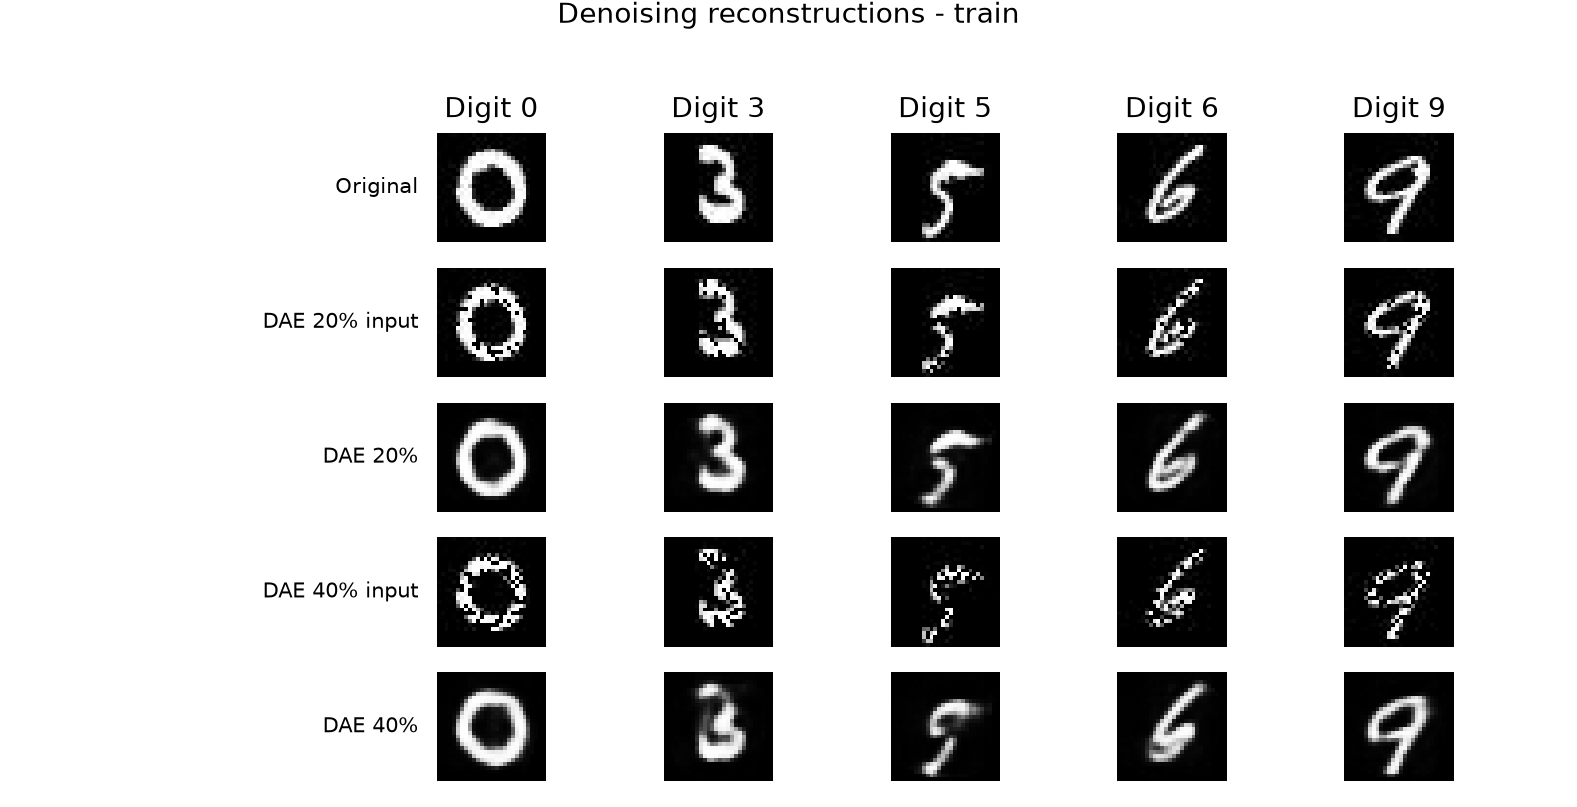
\includegraphics[width=\linewidth,height=0.70\textheight,keepaspectratio]{denoising_train.png}

\end{center}

{\small For every original image, the 20\% masked input and its reconstruction are followed by the 40\% masked input and its reconstruction. Both recover clean targets.}\par

\clearpage

\section{Task 5: val denoising examples}

\begin{center}

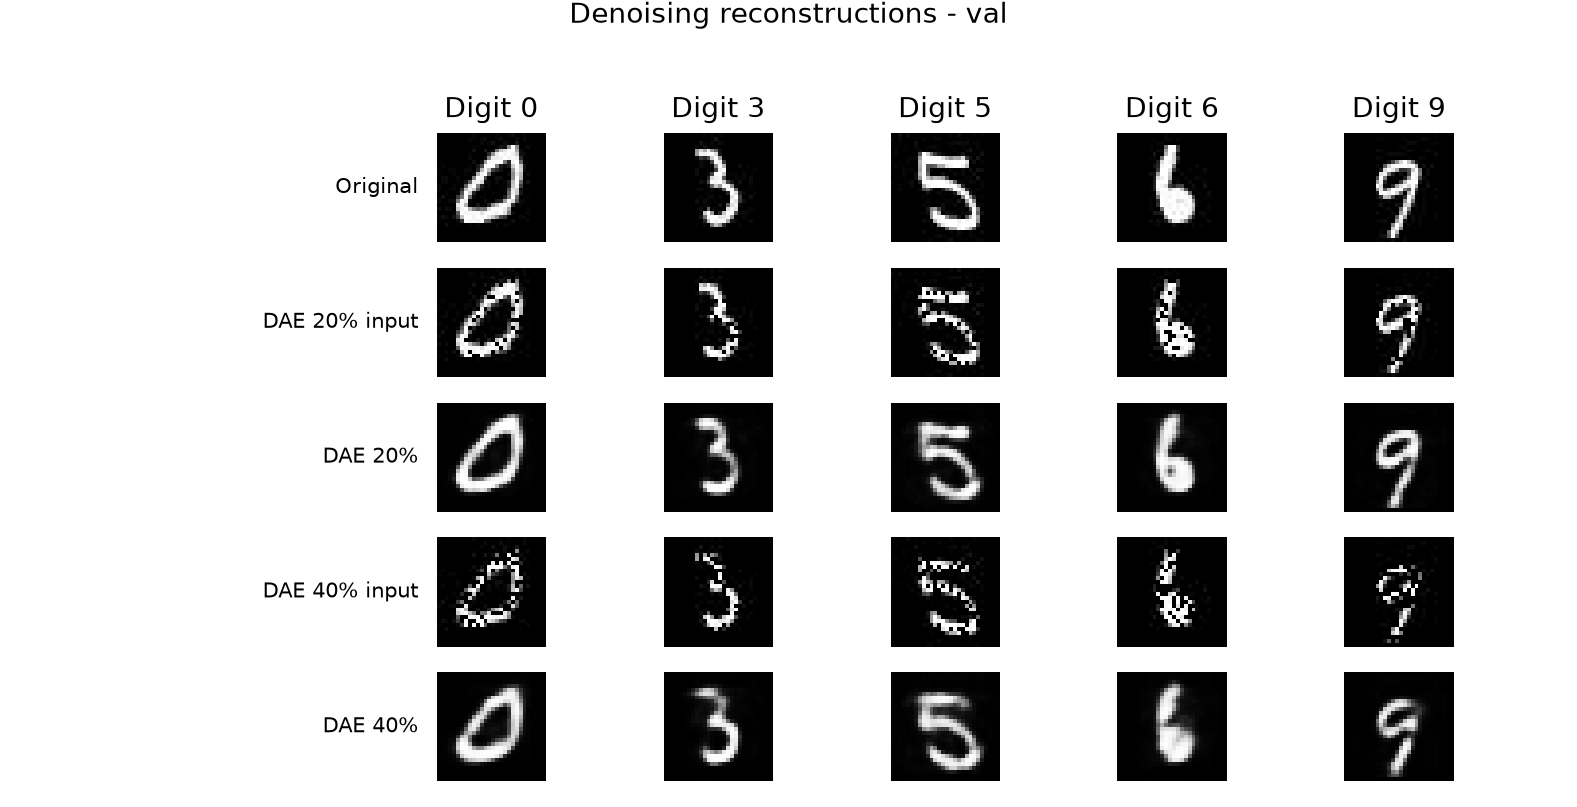
\includegraphics[width=\linewidth,height=0.70\textheight,keepaspectratio]{denoising_val.png}

\end{center}

{\small For every original image, the 20\% masked input and its reconstruction are followed by the 40\% masked input and its reconstruction. Both recover clean targets.}\par

\clearpage

\section{Task 5: test denoising examples}

\begin{center}

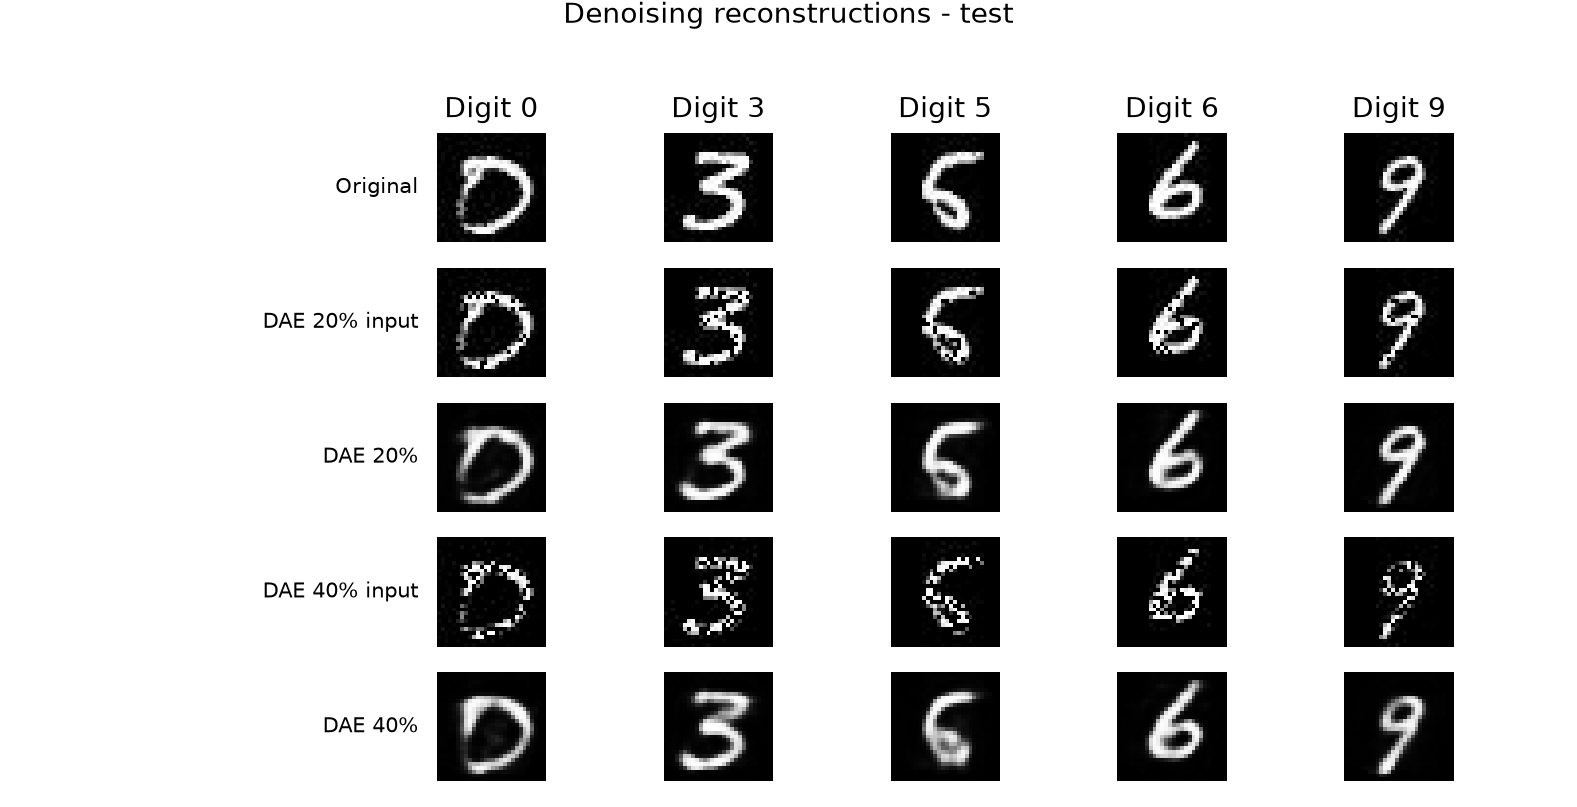
\includegraphics[width=\linewidth,height=0.70\textheight,keepaspectratio]{denoising_test.png}

\end{center}

{\small For every original image, the 20\% masked input and its reconstruction are followed by the 40\% masked input and its reconstruction. Both recover clean targets.}\par

\clearpage

\section{Task 6: encoder weight interpretation}

All 256 input-to-bottleneck weight vectors are reshaped to 28 $\times$ 28. Red denotes positive weights favoring bright pixels; blue denotes negative weights favoring dark pixels. The three grids share a symmetric color scale set by the pooled 99th percentile of absolute weights; biases are excluded.


Sigmoid activation is monotone in $w^Tx+b$, so the signed weight template shows a neuron's preferred input pattern, as requested in the assignment. Under $0\leq x_j\leq1$, an exact maximizing input has $x_j=1$ where $w_j>0$ and $x_j=0$ where $w_j<0$. The following figures display the assigned weight templates, not numerically optimized digit-like images.


\begingroup\small\setlength{\tabcolsep}{5pt}

\begin{tabularx}{\linewidth}{Yrrr}

\toprule

\textbf{Encoder} & \textbf{Weight RMS} & \textbf{Neighbor difference} & \textbf{Difference / RMS} \\

\midrule

shallow & 0.19207 & 0.15198 & 0.79125 \\

denoising\_20 & 0.20347 & 0.14085 & 0.69223 \\

denoising\_40 & 0.24188 & 0.14403 & 0.59547 \\

\bottomrule\end{tabularx}\endgroup\par\medskip

The neighbor difference averages absolute changes between adjacent horizontal and vertical weights; division by RMS removes overall weight scale. denoising\_40 has the smallest ratio in this run, indicating smoother local templates by this measure. This statistic is not classification accuracy. Neuron indices are not aligned between independently trained models, so comparisons should be at the set level.


\clearpage

\section{Task 6: clean shallow autoencoder}

\begin{center}

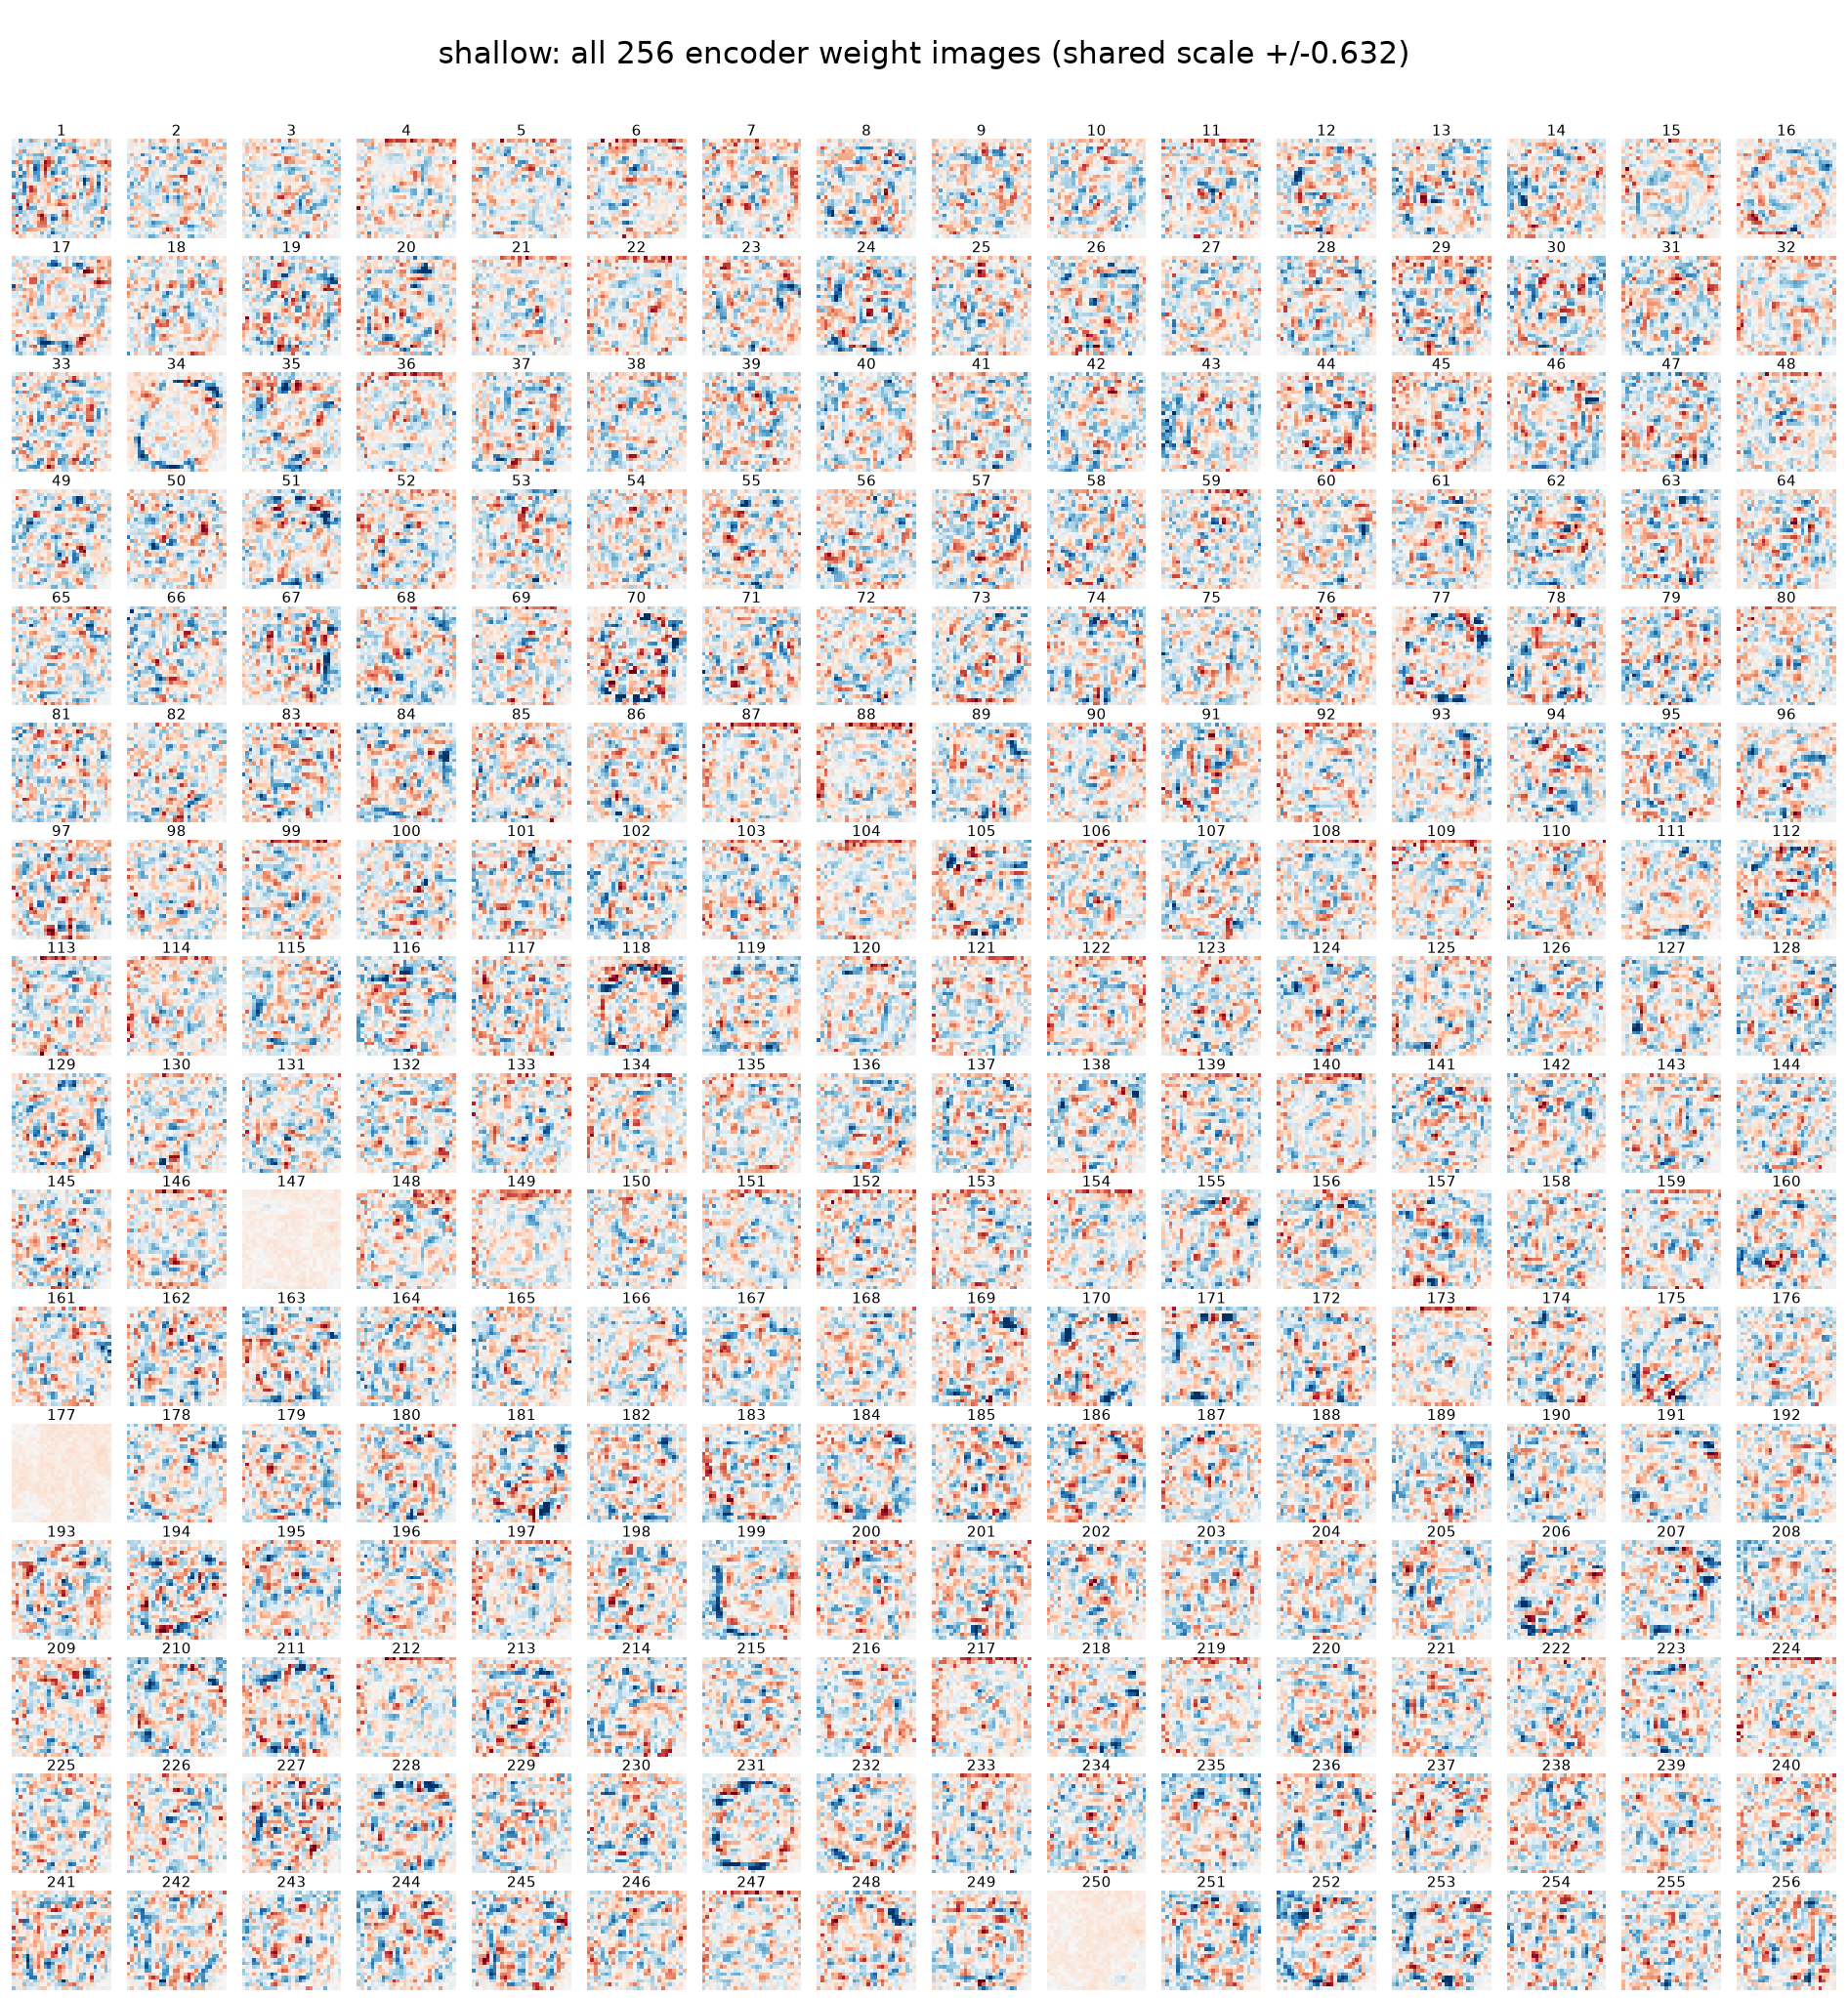
\includegraphics[width=\linewidth,height=0.81\textheight,keepaspectratio]{weights_shallow.png}

\end{center}

{\small Every neuron in the selected bottleneck is included, with one shared signed color scale. Numbers identify neurons within this model.}\par

\clearpage

\section{Task 6: 20 percent denoising autoencoder}

\begin{center}

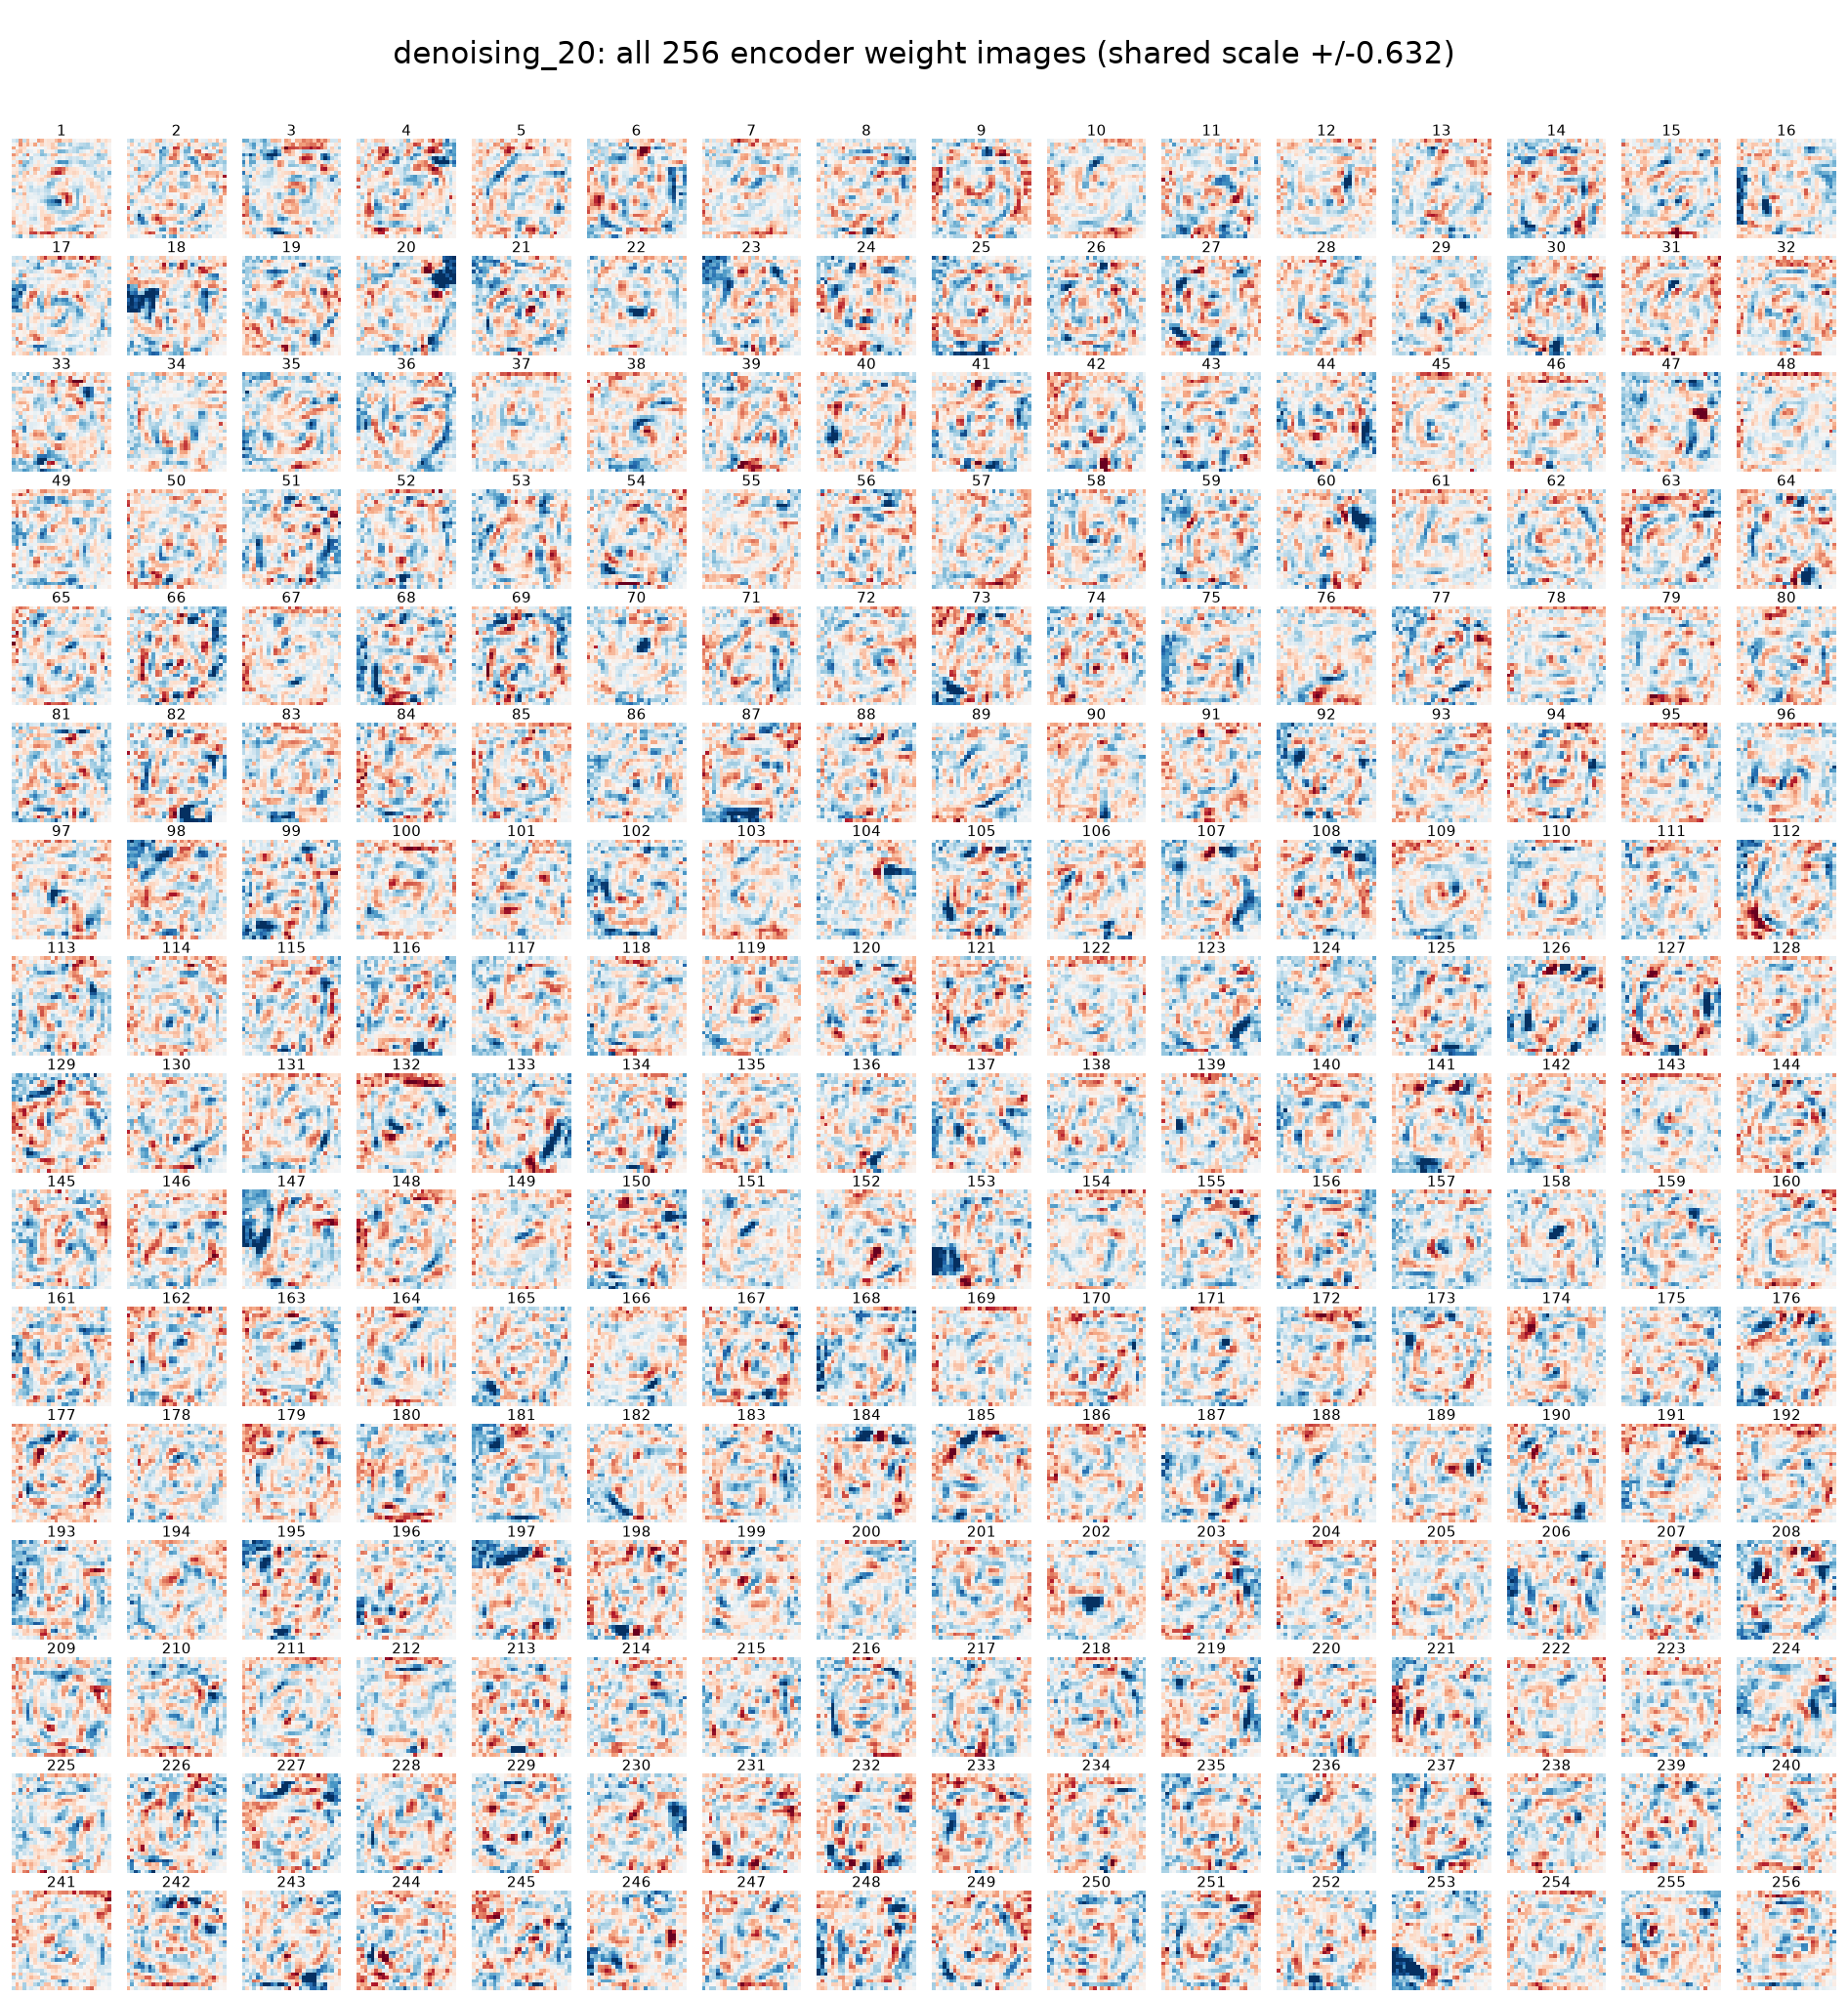
\includegraphics[width=\linewidth,height=0.81\textheight,keepaspectratio]{weights_denoising_20.png}

\end{center}

{\small Every neuron in the selected bottleneck is included, with one shared signed color scale. Numbers identify neurons within this model.}\par

\clearpage

\section{Task 6: 40 percent denoising autoencoder}

\begin{center}

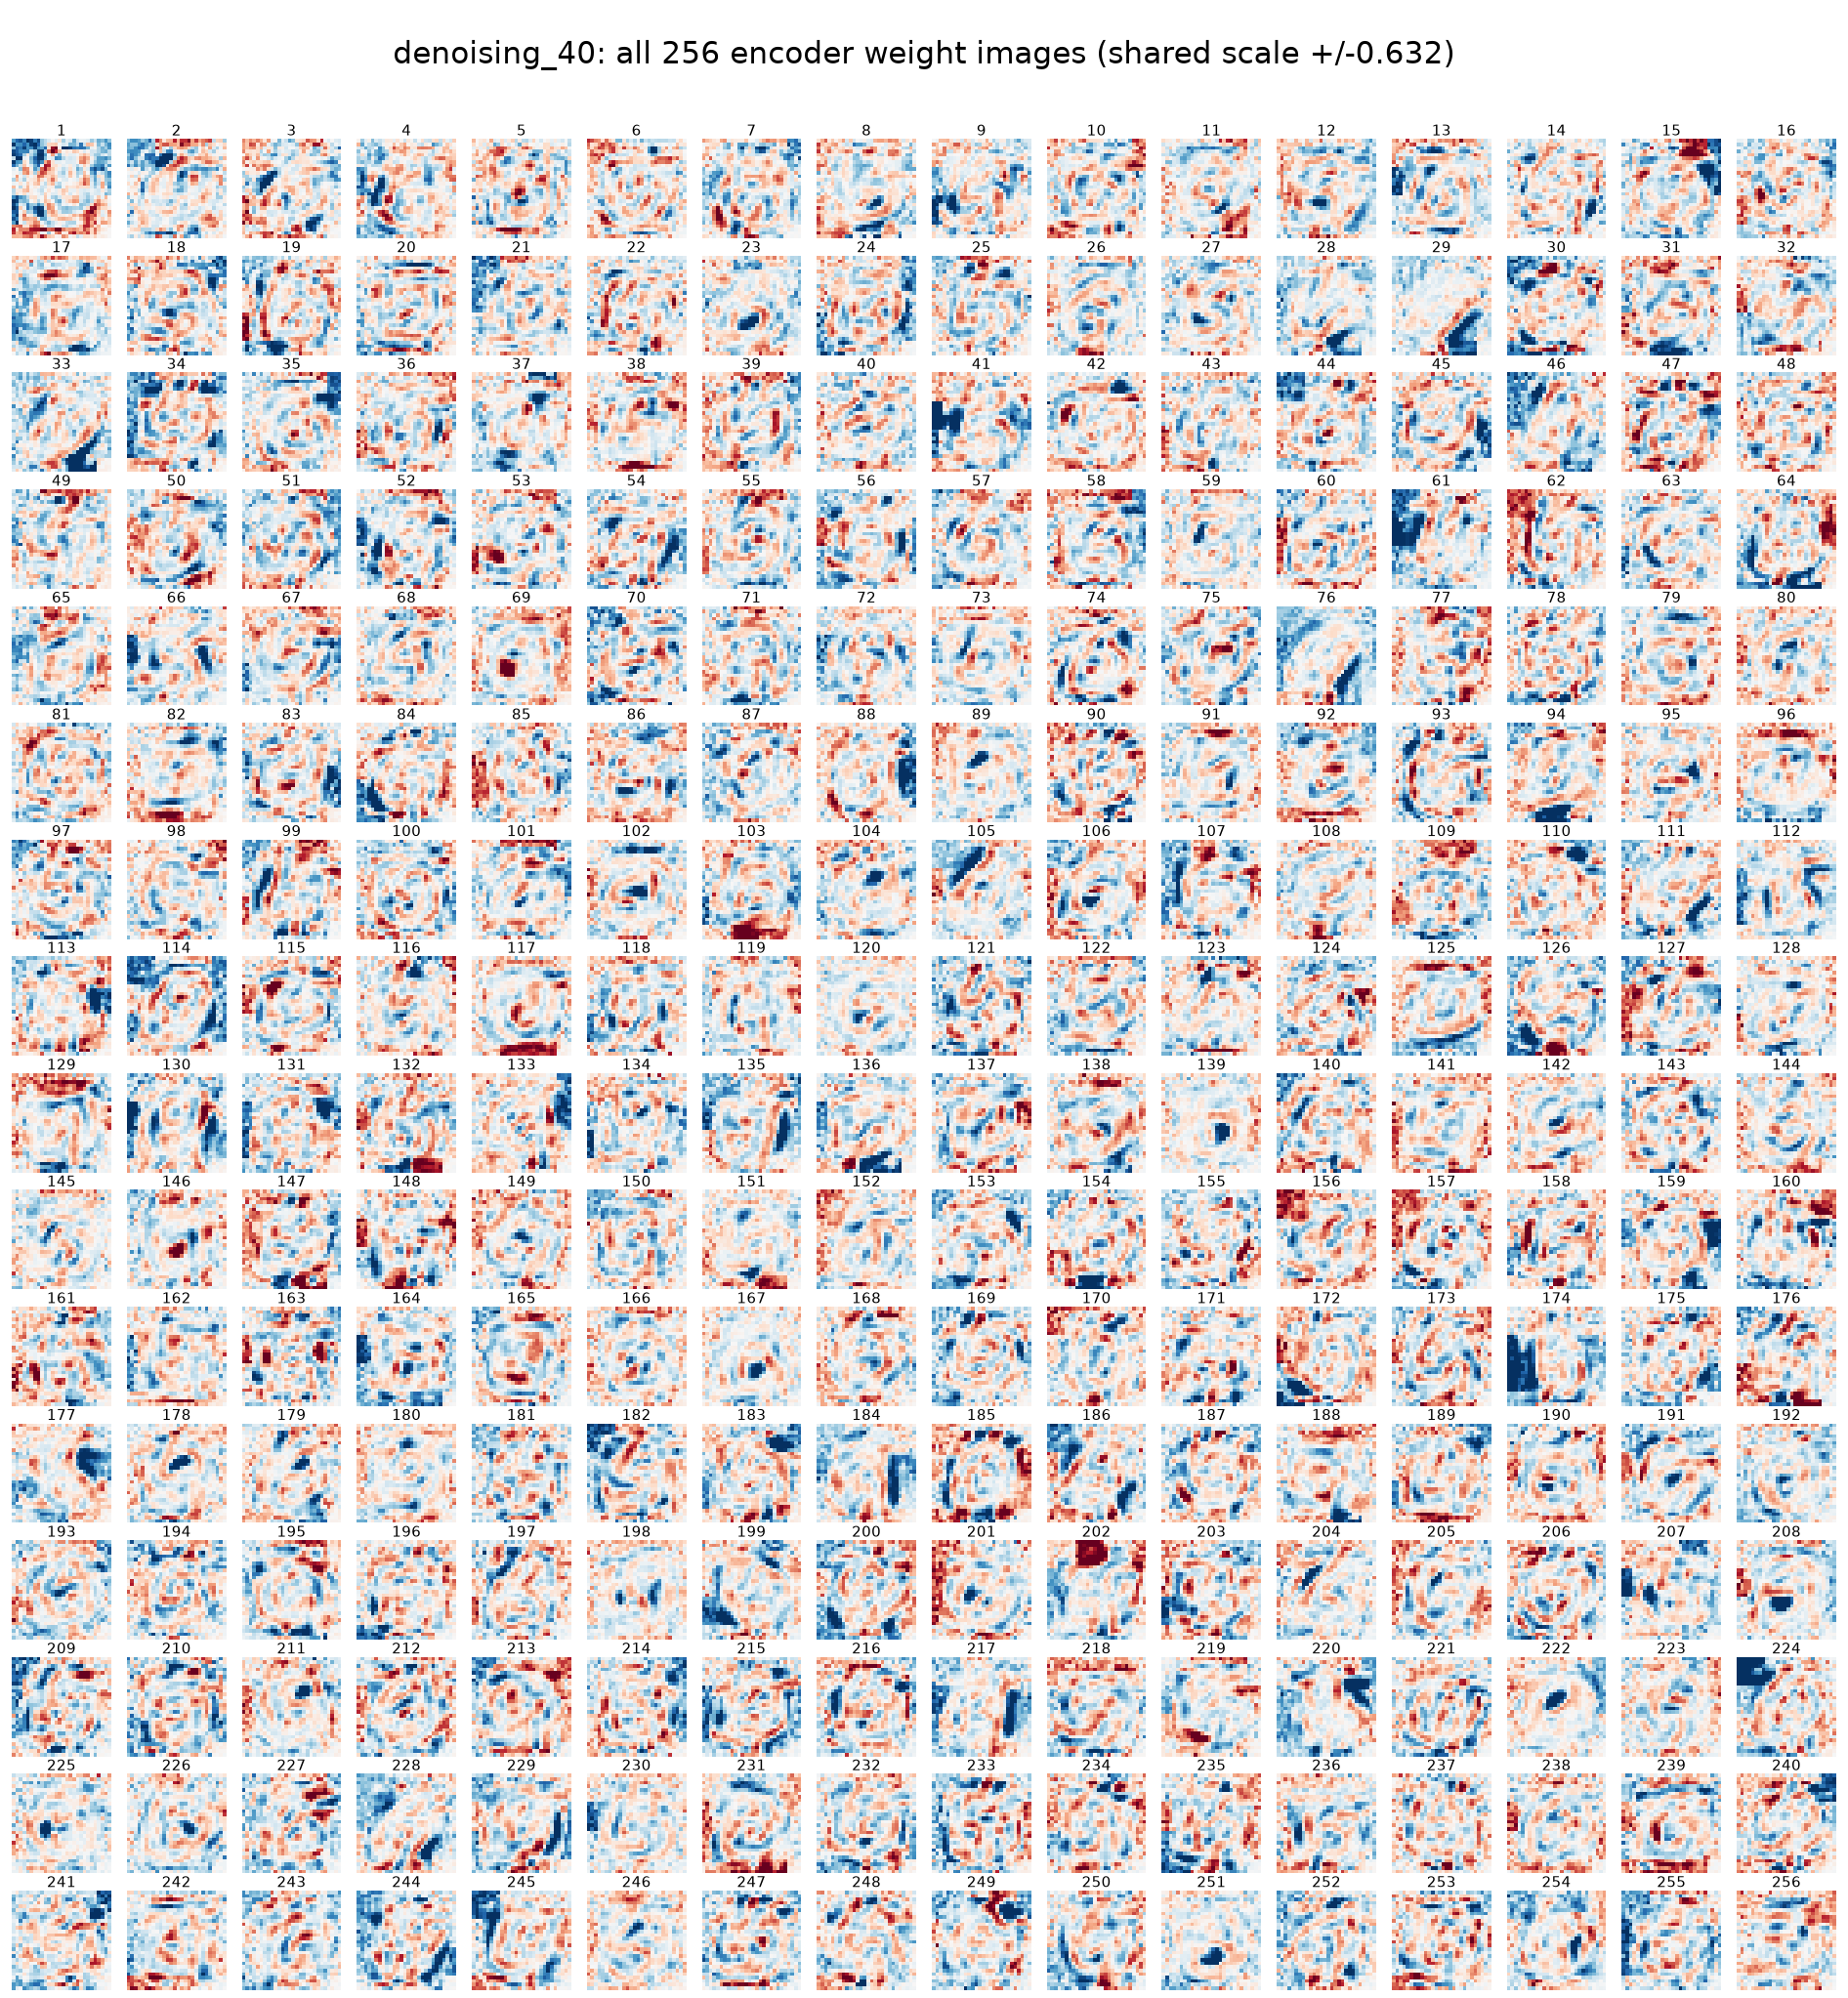
\includegraphics[width=\linewidth,height=0.81\textheight,keepaspectratio]{weights_denoising_40.png}

\end{center}

{\small Every neuron in the selected bottleneck is included, with one shared signed color scale. Numbers identify neurons within this model.}\par

\clearpage

\section{Comparison with Assignment 3}

\begingroup\small\setlength{\tabcolsep}{5pt}

\begin{tabularx}{\linewidth}{Yrlrrr}

\toprule

\textbf{Study} & \textbf{Dim.} & \textbf{Optimizer / FCNN} & \textbf{Val.} & \textbf{Test} & \textbf{Delta (pp)} \\

\midrule

Assignment 3 reproduction & 784 & NAG & 97.89\% & 97.87\% & 0.00 \\

PCA (Task 1) & 64 & 128 & 98.21\% & 98.18\% & +0.32 \\

Shallow AE (Task 3) & 256 & 128 $\to$ 64 & 98.21\% & 98.05\% & +0.18 \\

Deep AE (Task 4) & 256 & 128 & 98.63\% & 98.18\% & +0.32 \\

DAE, 20\% masking & 256 & 128 $\to$ 64 & 98.10\% & 97.71\% & -0.16 \\

DAE, 40\% masking & 256 & 128 $\to$ 64 & 98.16\% & 97.87\% & +0.00 \\

\bottomrule\end{tabularx}\endgroup\par\medskip

For Assignment 3 the middle column records its optimizer, and its full architecture is listed earlier. For Assignment 4 it records the FCNN hidden layers; all those FCNNs use Adam. The delta is test accuracy minus the Assignment 3 test accuracy, in percentage points. The best test-ranked dimension is reported within each Task 1, 3, or 4 representation family.


\begin{center}

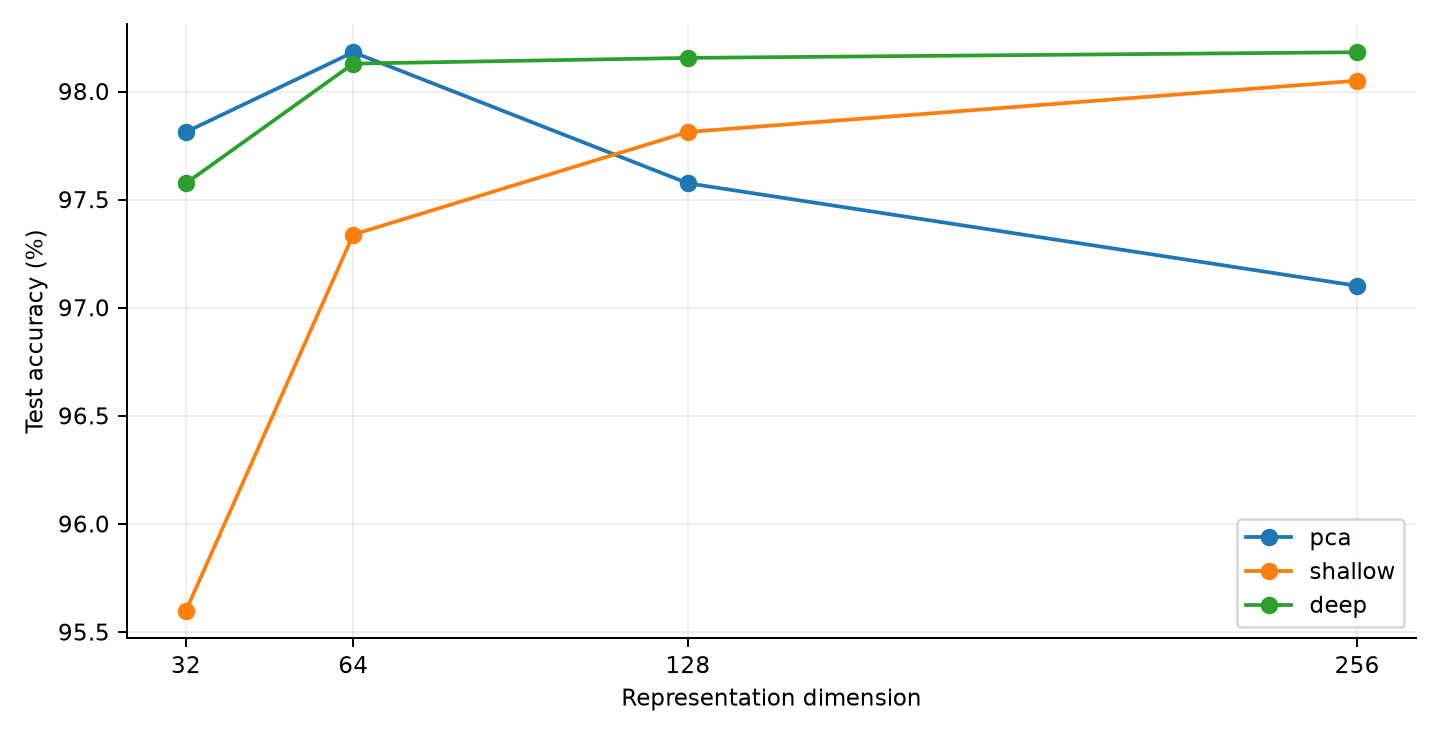
\includegraphics[width=\linewidth,height=0.34\textheight,keepaspectratio]{accuracy_comparison.png}

\end{center}

{\small At each dimension, the FCNN architecture was selected on validation accuracy. PCA, shallow AE, and deep AE classification are compared on the same test split.}\par

PCA reaches 98.18\%, while the deep AE reaches 98.18\% in this study. The best shallow result is 98.05\%. The numerical differences to Assignment 3 above are the requested comparison; they do not prove that a representation alone caused a performance difference, given the different architecture and training requirements.


\clearpage

\section{Learning behavior and observations}

\begin{center}

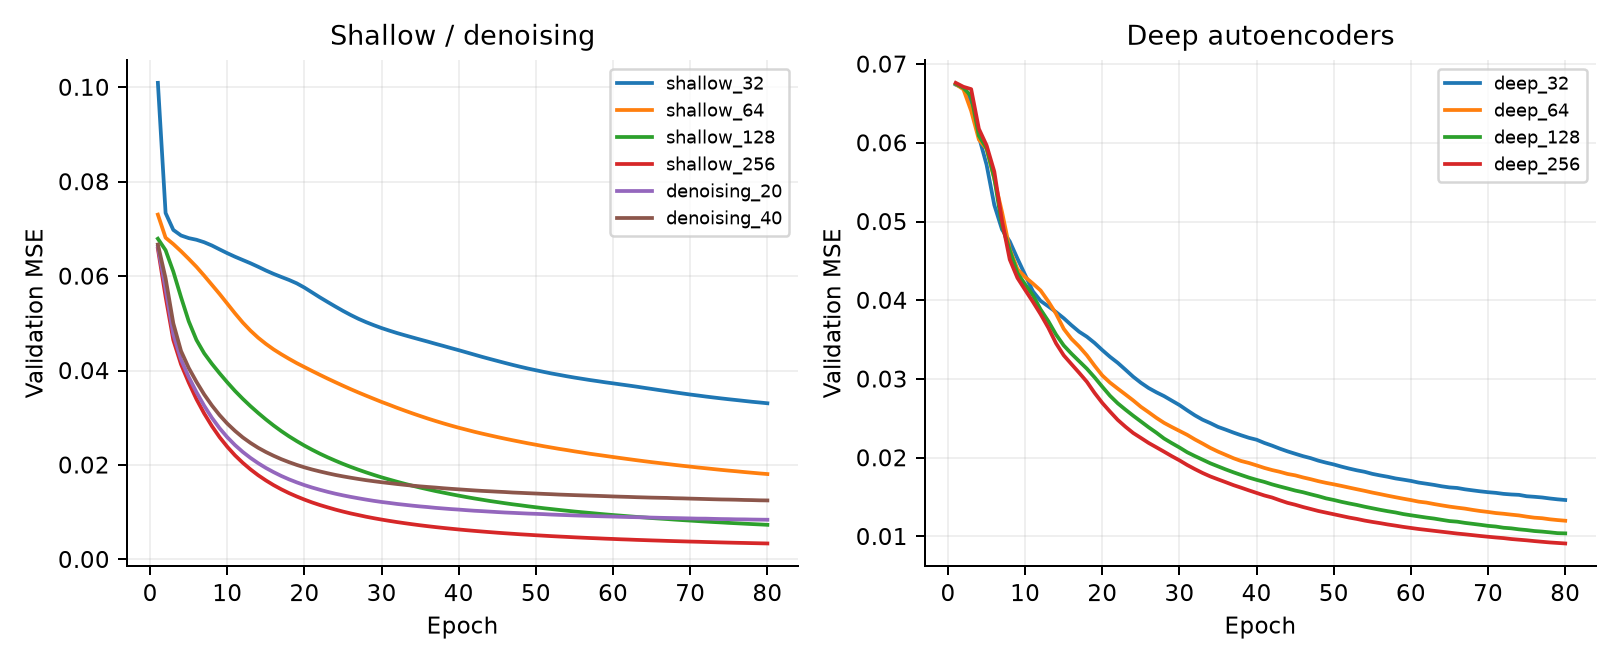
\includegraphics[width=\linewidth,height=0.37\textheight,keepaspectratio]{ae_learning_curves.png}

\end{center}

{\small Validation reconstruction MSE during AE training. Final split MSE values are separately recomputed after restoring the selected checkpoint.}\par

Shallow reconstruction error decreases strongly as bottleneck width grows in this run. The deep encoder improves classification over the shallow encoder at smaller widths, even though reconstruction MSE and classification accuracy are not interchangeable. A nonlinear representation can preserve useful digit structure without minimizing every pixel discrepancy.


Denoising encourages recovery from missing evidence. The weight smoothness statistics change with corruption training, but the measured reconstruction and clean/noisy classification results are the evidence of its effects. Increasing noise can alter both reconstruction fidelity and encoder adaptation; better classification is not guaranteed.


All AE curves were still improving over parts of the finite training budget. Therefore these results compare the stated training setup, not the maximum attainable performance of every architecture. The study uses one seed per experiment and does not supply confidence intervals or repeated-run significance tests.


\clearpage

\section{Specification notes and verification}

\textbf{Task 4 wording.} Its heading says `2-hidden layer autoencoder', while Task 2 specifies a three-hidden-layer autoencoder with 400 neurons in the first and third hidden layers. Task 4 uses the two-layer encoder $784\to400\to d$ of that explicitly specified deep autoencoder; no additional unspecified architecture is introduced.


\textbf{Test-informed denoising dimension.} Task 5 explicitly chooses its bottleneck by the best Task 3 test accuracy. This instruction is followed and recorded. Downstream test results therefore reuse test information during design; a fresh held-out split would be needed for an unbiased estimate after that choice.


\textbf{Checks.} Assignment 4 verification recomputes all ten AE reconstruction errors, saved latent samples, and the accuracies/confusion matrices for all 15 selected classifiers. PCA's training mean, component orthogonality, and projections are checked. Four pipeline tests cover train-only PCA fitting, required model shapes and sigmoid ranges, seeded corruption, and checkpoint restoration. Assignment 3 additionally checks every optimizer against PyTorch, matched initialization, the exact stopping condition, and final checkpoint metrics.


\textbf{Reproduce.} Run \texttt{python run\_assignment3.py} in the Assignment 3 folder, then use the saved \texttt{assignment3\_best.json} when reproducing the Assignment 4 study. \texttt{python report.py --compile} generates both LaTeX projects and compiles these PDFs. The projects contain their main \texttt{.tex} files and local figure assets, and work with pdfLaTeX or Overleaf.


Sources: \nolinkurl{CS601T_Assignment3_Details_07Sept2026.pdf} and \nolinkurl{CS601T_Assignment4_Details_30Sept2026.pdf}.


Dataset SHA-256: \texttt{d973de54462a8f8710f74cb65d7b5670}\\ \texttt{993802b9252e531d78aaee19d93cb2a8}.


\end{document}
